\documentclass[12pt,a4paper]{article}

% ================= PAQUETES =================
\usepackage[utf8]{inputenc}
\usepackage[T1]{fontenc}
\usepackage[spanish,es-tabla]{babel}
\usepackage{graphicx}
\usepackage{geometry}
\usepackage{fancyhdr}
\usepackage{listings}
\usepackage{xcolor}
\usepackage{float}
\usepackage{booktabs}
\usepackage{caption}
\usepackage{placeins}
\usepackage{amsmath}
\usepackage{tabularx}
\usepackage{rotating}
% Las páginas con sidewaysfigure/sidewaystable se marcan con /Rotate para que el visor las
% muestre horizontales (necesita dos pasadas de pdflatex; build.sh ya hace dos).
\makeatletter
\newcommand{\rotatepage}[1]{\global\@namedef{rotpage@#1}{}}
\newcommand{\markrotpage}{\protected@write\@auxout{}{\string\rotatepage{\thepage}}}
\AddToHook{shipout/before}{\ifcsname rotpage@\the\value{page}\endcsname
  \global\pdfpageattr{/Rotate 90}\else\global\pdfpageattr{}\fi}
\AtEndEnvironment{sidewaysfigure}{\markrotpage}
\AtEndEnvironment{sidewaystable}{\markrotpage}
\makeatother
\usepackage{microtype}
\usepackage{array}
\usepackage{multirow}

\emergencystretch=3em
\graphicspath{{figs/}}
\usepackage[hidelinks]{hyperref}
\usepackage{needspace}
\setlength{\parindent}{1.1em}
\setlength{\parskip}{0.18em}
\renewcommand{\arraystretch}{1.12}

% Programas en assembly (.s del repositorio)
\lstdefinelanguage{rvasm}{
  morecomment=[l]{;},
  morecomment=[l]{//},
  sensitive=false
}
\lstdefinestyle{programa}{
  language=rvasm,
  basicstyle=\ttfamily\scriptsize,
  commentstyle=\color{gray},
  numbers=left,
  numberstyle=\tiny\color{gray},
  numbersep=6pt,
  frame=single,
  xleftmargin=2em,
  framexleftmargin=1.5em,
  breaklines=true,
  columns=fullflexible,
  keepspaces=true,
  captionpos=b,
  aboveskip=1em,
  belowskip=1em,
  showstringspaces=false
}
% Fragmentos de Verilog
\lstdefinestyle{verilog}{
  language=Verilog,
  basicstyle=\ttfamily\scriptsize,
  keywordstyle=\color{blue!60!black}\bfseries,
  commentstyle=\color{gray},
  frame=single,
  xleftmargin=1em,
  framexleftmargin=0.5em,
  columns=fullflexible,
  breaklines=true,
  keepspaces=true,
  showstringspaces=false,
  captionpos=b,
  aboveskip=0.8em,
  belowskip=0.8em
}
\renewcommand{\lstlistingname}{Código}
\captionsetup[figure]{font=small,labelfont=bf,skip=5pt}
\captionsetup[table]{font=small,labelfont=bf,skip=5pt}
\captionsetup[lstlisting]{font=small,labelfont=bf}

\newcommand{\sig}[1]{\texttt{#1}}

% ================= MÁRGENES =================
\geometry{
  a4paper,
  margin=2.5cm,
  top=3.0cm,
  headheight=1.5cm,
  headsep=0.65cm
}

% ================= ENCABEZADO Y PIE =================
\pagestyle{fancy}
\fancyhf{}
\fancyhead[L]{
\includegraphics[height=1.15cm]{utec-logo.png}}
\fancyhead[R]{2026-2}
\fancyfoot[L]{Arquitectura de Computadoras (CS3051)}
\fancyfoot[R]{\thepage}
\renewcommand{\headrulewidth}{0.4pt}
\renewcommand{\footrulewidth}{0pt}

\begin{document}

% ================= PORTADA =================
\begin{center}
    
\includegraphics[height=10cm]{utec-logo.png}\\
    Arquitectura de Computadoras \\
    (CS3051) \\
    \vspace{1cm}
    {\large \textbf{Diseño e implementación de un procesador RISC-V superescalar Dual-Issue con optimización microarquitectónica}} \\
    \vspace{1cm}
    {\Large \textbf{Proyecto 2 - Entrega final}} \\
    \vspace{0.4cm}
    {\large Optimización: predicción dinámica de saltos con Branch Target Buffer y contador de 2 bits} \\
    \vspace{1cm}
    Alvarado León, Adriana Celeste \\
    Daza Yalta, Gino Jesús \\
    Ccolcca Flores, Marylin Regina \\
    \vspace{1.5cm}
    \textbf{Profesor:} Williams Valencia, Carlos Eduardo \\
    \vspace{0.5cm}
    16 de noviembre de 2026
\end{center}

\newpage
\thispagestyle{fancy}
\setcounter{tocdepth}{2}
{\small\setlength{\parskip}{0pt}\tableofcontents}
\newpage

% =====================================================================
\section{Introducción}

En las dos primeras entregas se construyó un procesador RISC-V RV32I \textbf{Dual-Issue In-Order}: dos vías de ejecución con una ALU cada una, un Register File de cuatro lecturas y dos escrituras, un único puerto de memoria de datos y una única unidad de resolución de saltos (\textit{Branch Unit}), con una Issue Unit que emite dos, una o ninguna instrucción por ciclo y reagrupa la instrucción que no pudo emitirse. En esta entrega final se agrega una \textbf{optimización microarquitectónica} sobre ese diseño y se evalúan experimentalmente las tres configuraciones que pide el enunciado:

\begin{itemize}
    \item \textbf{A}: pipeline Single-Issue de cinco etapas (\texttt{designs/pipeline}).
    \item \textbf{B}: Dual-Issue sin optimización (\texttt{designs/dualissue}), el procesador de E2.
    \item \textbf{C}: Dual-Issue con \textbf{predicción dinámica de saltos} mediante un \textit{Branch Target Buffer} (BTB) de 16 entradas con un contador saturado de 2 bits por entrada (\texttt{designs/dualissue-btb}).
\end{itemize}

El informe presenta la limitación que motiva la optimización (Sección~\ref{sec:fund}), el diseño y los módulos modificados (Sección~\ref{sec:diseno}), los testbenches y waveforms que validan la predicción (Sección~\ref{sec:valid}), los dos programas de comparación (Sección~\ref{sec:programas}) y la comparación cuantitativa y el análisis de las tres arquitecturas (Secciones~\ref{sec:comp} y~\ref{sec:analisis}). Los fragmentos de Verilog y los programas se incluyen directamente desde los archivos del repositorio.

% =====================================================================
\section{Fundamento de la optimización}
\label{sec:fund}

\subsection{Limitación del Dual-Issue: el costo de los saltos tomados}

En el procesador B los saltos se resuelven en Execute, y mientras tanto Fetch sigue buscando en secuencia: en la práctica predice siempre que el salto \emph{no} se toma. Cuando el salto se toma, la Hazard Unit descarta el par que está en Decode, el par que está en Fetch y, si el salto está en el slot~0, también su compañero del slot~1. Cada salto tomado cuesta entonces 2 ciclos, en los que se dejan de emitir hasta 4 instrucciones (Fig.~\ref{fig:pd-nopred}).

\begin{figure}[H]
    \centering
    \includegraphics[width=0.9\linewidth]{pd-nopred}
    \caption{Dual-Issue sin predicción (B): el \texttt{beq} tomado en EX descarta su compañero del slot~1 y los dos pares buscados detrás. La iteración del bucle dura cinco ciclos aunque solo tres emiten instrucciones útiles.}
    \label{fig:pd-nopred}
\end{figure}

La comparación preliminar de E2 ya identificaba a los saltos como la principal causa de que el IPC quedara lejos de 2. Las mediciones de esta entrega lo confirman en los programas con bucles:

\begin{itemize}
    \item En el \textbf{programa del profesor}, B ejecuta 68 saltos tomados: $2 \times 68 = 136$ de sus 387 ciclos (35\,\%) se pierden por flush.
    \item En el \textbf{programa propio} (\textit{bubble sort}), 199 saltos tomados cuestan 398 de 1421 ciclos (28\,\%).
\end{itemize}

\noindent El problema crece con el ancho de emisión: en el pipeline un salto tomado desperdicia 2 instrucciones, en el Dual-Issue hasta 4. Es además una limitación que la Issue Unit no puede resolver, porque no depende de las dependencias entre instrucciones sino de que Fetch no sabe a dónde ir hasta que el salto llega a Execute.

\subsection{Propuesta: predicción dinámica con BTB y contador de 2 bits}

La optimización aprobada es un \textbf{predictor dinámico de saltos} en Fetch. En cada ciclo, el BTB se consulta con los PC de las dos instrucciones del par; si una de ellas es un salto conocido y su contador predice ``tomado'', el siguiente PC pasa a ser el destino guardado, sin esperar a Execute. El salto se sigue resolviendo en la Branch Unit, que ahora además \emph{verifica} la predicción: solo si falla se descartan las instrucciones jóvenes y se corrige el PC.

\begin{table}[H]
\centering
\small
\begin{tabularx}{\linewidth}{lX}
\toprule
\textbf{Aspecto} & \textbf{Propuesta} \\
\midrule
Nombre & Predicción dinámica de saltos: BTB de correspondencia directa con contador de 2 bits. \\
Limitación & Cada salto tomado cuesta 2 ciclos y hasta 4 instrucciones, porque Fetch predice siempre ``no tomado''. \\
Modificación & BTB en Fetch (2 lecturas, 1 escritura), cadena del siguiente PC con los destinos predichos, anulación del slot~1, transporte de la predicción hasta EX, verificación en la Branch Unit y flush por \emph{error de predicción} en lugar de por \emph{salto tomado}. \\
Módulos & \texttt{btb.v} (nuevo), \texttt{datapath.v}, \texttt{branchunit.v}, \texttt{hazard.v}, \texttt{riscv.v}. \\
Métricas & Ciclos, IPC, CPI, speedup frente a A y B, errores de predicción, precisión, aciertos en el BTB y ciclos de flush. \\
\bottomrule
\end{tabularx}
\caption{Resumen de la propuesta de optimización.}
\label{tab:propuesta}
\end{table}

Se eligió el contador de 2 bits frente a uno de 1 bit porque en un bucle el de 1 bit se equivoca dos veces por ejecución (a la salida y en la primera iteración de la siguiente), mientras que el de 2 bits tolera un único resultado contrario y se equivoca solo a la salida. El BTB es necesario porque en Fetch la instrucción todavía no está decodificada: no se sabe si es un salto ni cuál es su destino, y lo único disponible es su PC.

Si la predicción acierta, el salto no cuesta nada (Fig.~\ref{fig:pd-pred}); si falla, se paga la misma penalización de 2 ciclos que hoy paga cada salto tomado. La optimización nunca empeora un salto que en B no se toma \emph{y} que el contador predice como no tomado; puede empeorar los saltos cuyo comportamiento cambia en cada ejecución (Sección~\ref{sec:cuando}).

\begin{figure}[H]
    \centering
    \includegraphics[width=0.9\linewidth]{pd-pred-slot0}
    \caption{El mismo bucle con predicción (C): el \texttt{beq} del slot~0 se predice tomado en Fetch, su compañero se anula y la iteración baja de cinco a tres ciclos.}
    \label{fig:pd-pred}
\end{figure}

% =====================================================================
\section{Diseño e implementación}
\label{sec:diseno}

\subsection{Organización general}

La Figura~\ref{fig:top} muestra la integración de los módulos de C. Respecto a B, el BTB se agrega dentro de la etapa Fetch del datapath; la Branch Unit le devuelve las señales de actualización y entrega a Fetch y a la Hazard Unit \sig{MispredictE}, \sig{PCCorrectE} y \sig{FlushLane1E}. La Issue Unit, el forwarding, el Register File, la memoria de datos y el Controller no cambian. La Figura~\ref{fig:proc} presenta el datapath completo; los elementos nuevos aparecen en café.

\begin{figure}[H]
    \centering
    \includegraphics[width=\linewidth]{dualissue-btb-top}
    \caption{Integración de los módulos del procesador C (Dual-Issue + BTB).}
    \label{fig:top}
\end{figure}


\subsection{Contador de 2 bits}

Cada entrada del BTB tiene un contador saturado (Fig.~\ref{fig:fsm}). Los estados \texttt{11} y \texttt{10} predicen tomado y los estados \texttt{01} y \texttt{00} no tomado: la predicción es el bit más significativo. Un salto tomado incrementa el contador y uno no tomado lo decrementa, saturando en los extremos. Cuando un \texttt{beq} se toma por primera vez, su entrada se crea en \texttt{10} (\textit{weakly taken}); un \texttt{jal} siempre se toma, así que su entrada se crea directamente en \texttt{11}.

\begin{figure}[H]
    \centering
    \includegraphics[width=0.85\linewidth]{fsm-2bit}
    \caption{Contador de 2 bits. En café, el valor con que se crea la entrada de un \texttt{beq}.}
    \label{fig:fsm}
\end{figure}

\begin{sidewaysfigure}
    \centering
    \includegraphics[width=\linewidth,height=13.5cm,keepaspectratio]{proc-btb}
    \caption{Datapath del procesador Dual-Issue con predicción de saltos. En café: BTB, cadena del siguiente PC, reagrupamiento y anulación de la predicción, \{Pred, Target\} hasta la Branch Unit, \sig{PCCorrectE} y actualización del BTB.}
    \label{fig:proc}
\end{sidewaysfigure}


\subsection{Branch Target Buffer}

El BTB (\texttt{btb.v}) tiene 16 entradas de correspondencia directa. El índice son los bits $\sig{PC}[5{:}2]$ y cada entrada guarda un bit de validez V, el Tag $\sig{PC}[31{:}6]$ (26 bits), el contador (2 bits) y el destino (32 bits): 61 bits por entrada, 976 bits en total. Como Tag e índice forman el PC completo, un acierto identifica exactamente a la instrucción, y como solo se escriben saltos, una entrada válida implica que la instrucción es un salto:
\begin{equation}
\sig{predtaken} = \sig{V} \land (\sig{Tag} = \sig{PC}[31{:}6]) \land \sig{Ctr}[1]
\end{equation}
Tiene dos puertos de lectura combinacionales, uno por slot (\sig{PCF} y \sig{PCPlus4F}), y un puerto de escritura en el flanco de subida que maneja la Branch Unit desde Execute (Fig.~\ref{fig:btb}). Un salto tomado escribe la entrada (V, Tag, destino y contador); un salto no tomado con acierto solo decrementa el contador; un salto no tomado sin entrada no escribe nada.

\begin{figure}[H]
    \centering
    \includegraphics[width=\linewidth]{btb-inside}
    \caption{Estructura interna del BTB: dos puertos de lectura y el bloque de escritura.}
    \label{fig:btb}
\end{figure}

\lstinputlisting[style=verilog,firstline=27,lastline=65,caption={Lectura (Fetch) y actualización (Execute) del BTB (\texttt{btb.v}).},label={lst:btb}]{../../designs/dualissue-btb/btb.v}

\noindent La actualización lee el contador actual de la tabla y no una copia tomada en Fetch: en un bucle de dos pares, la instancia siguiente del mismo salto se busca antes de que la anterior se escriba, y una copia de Fetch estaría desactualizada.

\subsection{Fetch con predicción}

El siguiente PC se elige con una cadena de multiplexores con esta prioridad (Fig.~\ref{fig:fetch}):
\begin{equation*}
\sig{PCNextF} =
\begin{cases}
\sig{PCCorrectE} & \text{si } \sig{MispredictE} \quad\text{(error de predicción en EX)}\\
\sig{TargetF\_0} & \text{si } \sig{PredF\_0} \quad\text{(slot~0 predicho tomado)}\\
\sig{PCPlus4F}   & \text{si } \sig{RegroupD} \quad\text{(emisión parcial)}\\
\sig{TargetF\_1} & \text{si } \sig{PredF\_1} \quad\text{(slot~1 predicho tomado)}\\
\sig{PCPlus8F}   & \text{en otro caso}
\end{cases}
\end{equation*}
\sig{MispredictE} va primero porque, ante un error en EX, todo lo que está en F y D es del camino incorrecto. \sig{PredF\_0} va antes que \sig{RegroupD} porque durante un reagrupamiento \sig{InstrF\_0} pasa al slot~1 y, si es un salto predicho, lo que le sigue en el camino predicho es su destino. \sig{RegroupD} va antes que \sig{PredF\_1} porque durante un reagrupamiento \sig{InstrF\_1} se descarta y se vuelve a buscar.

Si el slot~0 buscado es un salto predicho tomado, el slot~1 es la instrucción siguiente en memoria y queda fuera del camino predicho: se anula antes de entrar a IF/ID con $\sig{AnnulF\_1} = \sig{PredF\_0} \land \lnot\sig{RegroupD}$. La predicción del slot~1 se reagrupa junto con su instrucción, con los mismos multiplexores que el par.

\noindent\begin{minipage}{\linewidth}
\lstinputlisting[style=verilog,firstline=84,lastline=89,caption={Cadena de prioridad del siguiente PC (\texttt{datapath.v}).},label={lst:pcnext}]{../../designs/dualissue-btb/datapath.v}
\end{minipage}

\noindent\begin{minipage}{\linewidth}
\lstinputlisting[style=verilog,firstline=116,lastline=128,caption={Anulación del slot~1 y reagrupamiento de la predicción (\texttt{datapath.v}).},label={lst:annul}]{../../designs/dualissue-btb/datapath.v}
\end{minipage}


\begin{figure}[H]
    \centering
    \includegraphics[height=12cm]{proc-btb-zoom-fetch}
    \caption{Fetch con predicción: BTB, cadena del siguiente PC, reagrupamiento de \{Pred, Target\} y anulación del slot~1.}
    \label{fig:fetch}
\end{figure}

\subsection{Transporte de la predicción}

La predicción se hace en Fetch y se verifica en Execute, así que viaja con la instrucción por los registros de pipeline: 33 bits por instrucción (\sig{Pred} y \sig{Target}). IF/ID crece de 192 a 258 bits y cada ID/EX de 207 a 240 bits. Como viaja en los mismos registros, obedece a los mismos stalls, flushes y reagrupamientos que su instrucción.

\subsection{Verificación en la Branch Unit}

La Branch Unit sigue seleccionando los operandos de la vía que tiene el salto (\sig{BrLaneE}), comparando y calculando \sig{PCTargetE}. Con los mismos multiplexores toma la predicción de esa vía y detecta el error de predicción, de dirección o de destino:
\begin{align}
\sig{MispredictE} &= \sig{CtrlE} \land \bigl[(\sig{PCSrcE} \neq \sig{PredTakenE}) \nonumber\\
&\qquad\quad \lor (\sig{PCSrcE} \land \sig{PCTargetE} \neq \sig{PredTargetE})\bigr] \\
\sig{PCCorrectE} &= \sig{PCSrcE}\ ?\ \sig{PCTargetE} : \sig{PCPlus4E} \\
\sig{FlushLane1E} &= \sig{MispredictE} \land \lnot\sig{BrLaneE}
\end{align}
El caso nuevo es el salto predicho tomado que no se toma: Fetch debe volver a $\sig{PC}+4$ del salto, por eso la Branch Unit recibe ahora el \sig{PCPlus4E} de cada vía (Fig.~\ref{fig:bu}).

\begin{figure}[H]
    \centering
    \includegraphics[width=\linewidth]{bu-inside}
    \caption{Branch Unit con verificación de la predicción y señales de actualización del BTB.}
    \label{fig:bu}
\end{figure}

\noindent\begin{minipage}{\linewidth}
\lstinputlisting[style=verilog,firstline=59,lastline=71,caption={Verificación de la predicción (\texttt{branchunit.v}).},label={lst:bu}]{../../designs/dualissue-btb/branchunit.v}
\end{minipage}

\subsection{Cambios en la Hazard Unit}

La Hazard Unit conserva su estructura; solo cambia la señal que indica que el camino es incorrecto: \sig{PCSrcE} (salto tomado) se reemplaza por \sig{MispredictE} (predicción incorrecta) y \sig{TakenE\_0} por \sig{FlushLane1E}. Un salto bien predicho ya no genera flush, y un salto predicho tomado que no se toma sí lo genera.

\begin{table}[H]
\centering
\small
\begin{tabular}{lll}
\toprule
\textbf{Señal} & \textbf{B: Dual-Issue} & \textbf{C: con predicción} \\
\midrule
\sig{lwStallD} & \sig{LoadUseD\_0} $\land\lnot$\sig{PCSrcE} & \sig{LoadUseD\_0} $\land\lnot$\sig{MispredictE} \\
\sig{RegroupD} & \sig{IssueOneD} $\land\lnot$\sig{lwStallD} $\land\lnot$\sig{PCSrcE} & \sig{IssueOneD} $\land\lnot$\sig{lwStallD} $\land\lnot$\sig{MispredictE} \\
\sig{FlushD} & \sig{PCSrcE} & \sig{MispredictE} \\
\sig{FlushE\_0} & \sig{lwStallD} $\lor$ \sig{PCSrcE} & \sig{lwStallD} $\lor$ \sig{MispredictE} \\
\sig{FlushE\_1} & \sig{lwStallD} $\lor$ \sig{PCSrcE} $\lor$ \sig{IssueOneD} & \sig{lwStallD} $\lor$ \sig{MispredictE} $\lor$ \sig{IssueOneD} \\
\sig{FlushM\_1} & \sig{TakenE\_0} & \sig{FlushLane1E} \\
\bottomrule
\end{tabular}
\caption{Salidas de la Hazard Unit en B y en C.}
\label{tab:hazard}
\end{table}

\noindent\begin{minipage}{\linewidth}
\lstinputlisting[style=verilog,firstline=50,lastline=65,caption={Stalls, reagrupamiento y flushes con predicción (\texttt{hazard.v}).},label={lst:hazard}]{../../designs/dualissue-btb/hazard.v}
\end{minipage}

\subsection{Módulos modificados y costo de hardware}

\begin{table}[H]
\centering
\small
\begin{tabularx}{\linewidth}{lX}
\toprule
\textbf{Módulo} & \textbf{Cambio respecto a B} \\
\midrule
\texttt{btb.v} & \textbf{Nuevo.} 16 entradas $\times$ 61 bits, 2 puertos de lectura, 1 de escritura; tamaño parametrizable (\texttt{IDXW}). \\
\texttt{datapath.v} & Instancia el BTB; cadena de 4 multiplexores 2:1 del siguiente PC; \sig{AnnulF\_1}; reagrupamiento de \{Pred, Target\}; IF/ID +66 bits, ID/EX +33 bits por vía; conexiones de la Branch Unit. \\
\texttt{branchunit.v} & Selección de \sig{PredE}, \sig{TargetE} y \sig{PCPlus4E} de la vía del salto; \sig{MispredictE} (un comparador de 32 bits más), \sig{PCCorrectE}, \sig{FlushLane1E} y salidas de actualización del BTB. \\
\texttt{hazard.v} & \sig{PCSrcE} $\to$ \sig{MispredictE}, \sig{TakenE\_0} $\to$ \sig{FlushLane1E}. \\
\texttt{riscv.v} & Conecta las nuevas señales entre datapath y Hazard Unit. \\
\bottomrule
\end{tabularx}
\caption{Módulos nuevos y modificados para la optimización. \texttt{issue.v}, \texttt{controller.v}, \texttt{regfile.v}, la ALU, las memorias y los demás módulos son idénticos a los de B.}
\label{tab:modulos}
\end{table}

En almacenamiento, la optimización agrega 976 bits del BTB y 132 bits de registros de pipeline. En lógica: dos comparadores de Tag de 26 bits y dos multiplexores 16:1 de 33 bits para las lecturas, el decodificador de escritura, un comparador de 32 bits para el destino predicho y siete multiplexores 2:1 (cuatro del siguiente PC, tres de la Branch Unit). No se sintetizó el diseño, por lo que la comparación supone el mismo periodo de reloj en las tres arquitecturas; la Sección~\ref{sec:limit} discute el impacto posible en la frecuencia.

% =====================================================================
\section{Testbenches y validación de la optimización}
\label{sec:valid}

\subsection{Infraestructura de pruebas}

\begin{itemize}
    \item \texttt{tb/perf\_tb.v}: un mismo testbench para las tres arquitecturas (\texttt{-DDUAL}, \texttt{-DOPT}). Cuenta ciclos desde el primer ciclo después del reset hasta que el \textit{halt} (\texttt{jal x0,0}) llega a WB, instrucciones retiradas, ciclos con doble emisión, stalls, reagrupamientos, flushes y, para los saltos en Execute, ejecuciones, tomados, errores de predicción y aciertos en el BTB. Al final imprime los 31 registros y la memoria de datos.
    \item \texttt{tb/run\_all.sh}: corre todos los programas en A, B y C, compara el estado final (registros y memoria) de las tres y reporta ciclos, IPC y speedups.
    \item \texttt{latex/informe-final/waves/final\_tb.v} (nuevo): comprueba las etapas A--D del programa del profesor contra los estados de referencia del enunciado (Sección~\ref{sec:prof}), calcula las métricas excluyendo el bucle \texttt{fin} y, con \texttt{+trace}, genera la traza ciclo a ciclo de la que se dibujan las waveforms.
\end{itemize}

\subsection{Programas de prueba de la optimización}

Se escribieron siete programas específicos (\texttt{tb/programs/opt/}), cada uno con los valores esperados en su encabezado. En los siete, el estado final de C coincide con esos valores y con el de A y B.

\begin{table}[H]
\centering
\small
\begin{tabularx}{\linewidth}{lXcc}
\toprule
\textbf{Programa} & \textbf{Caso que verifica} & \textbf{Err. B} & \textbf{Err. C} \\
\midrule
\texttt{pred\_slot0} & Salto predicho en el slot~0: anulación del slot~1, error a la salida y retorno a PC+4. & 10 & 3 \\
\texttt{pred\_slot1} & Salto predicho en el slot~1: el slot~0, más antiguo, se conserva. & 11 & 3 \\
\texttt{pred\_regroup} & Salto predicho que se reagrupa por RAW con la primera instrucción de su destino. & 6 & 3 \\
\texttt{pred\_jal} & \texttt{jal} en el BTB (contador 11) y salto hacia adelante que solo se toma una vez. & 12 & 4 \\
\texttt{pred\_pattern} & Patrón T, T, N: un error por periodo; el no tomado mal predicho retoma en PC+4. & 15 & 7 \\
\texttt{pred\_loaduse} & Stall por load-use detrás de un salto bien predicho. & 4 & 3 \\
\texttt{pred\_alias} & Dos saltos con el mismo índice del BTB que se reemplazan: solo fallos, nunca un resultado incorrecto. & 15 & 15 \\
\bottomrule
\end{tabularx}
\caption{Programas de prueba de la optimización. \textit{Err.}: errores de predicción (en B, todo salto tomado), incluido el \textit{halt}.}
\label{tab:opt-tests}
\end{table}

\noindent Las waveforms de esta sección son de la arquitectura C. El ciclo 1 es el primer ciclo después del reset, la misma numeración que usan los contadores de \texttt{perf\_tb}. Las direcciones se muestran en decimal, como en los listados de los programas; \sig{PC salto (E)} es el PC de la vía que ocupa la Branch Unit y \sig{Ctr (BTB)} el contador que tiene en ese momento la entrada de ese salto.

% ---------------------------------------------------------------------
\subsection{Prueba 1: salto en el slot 0}


Como referencia, la Figura~\ref{fig:w-slot0-B} muestra el programa en B: cada \texttt{beq} tomado produce dos ciclos vacíos en EX y cada iteración dura 5 ciclos. La Figura~\ref{fig:w-slot0} muestra la misma prueba en C.

\begin{figure}[H]
  \centering
  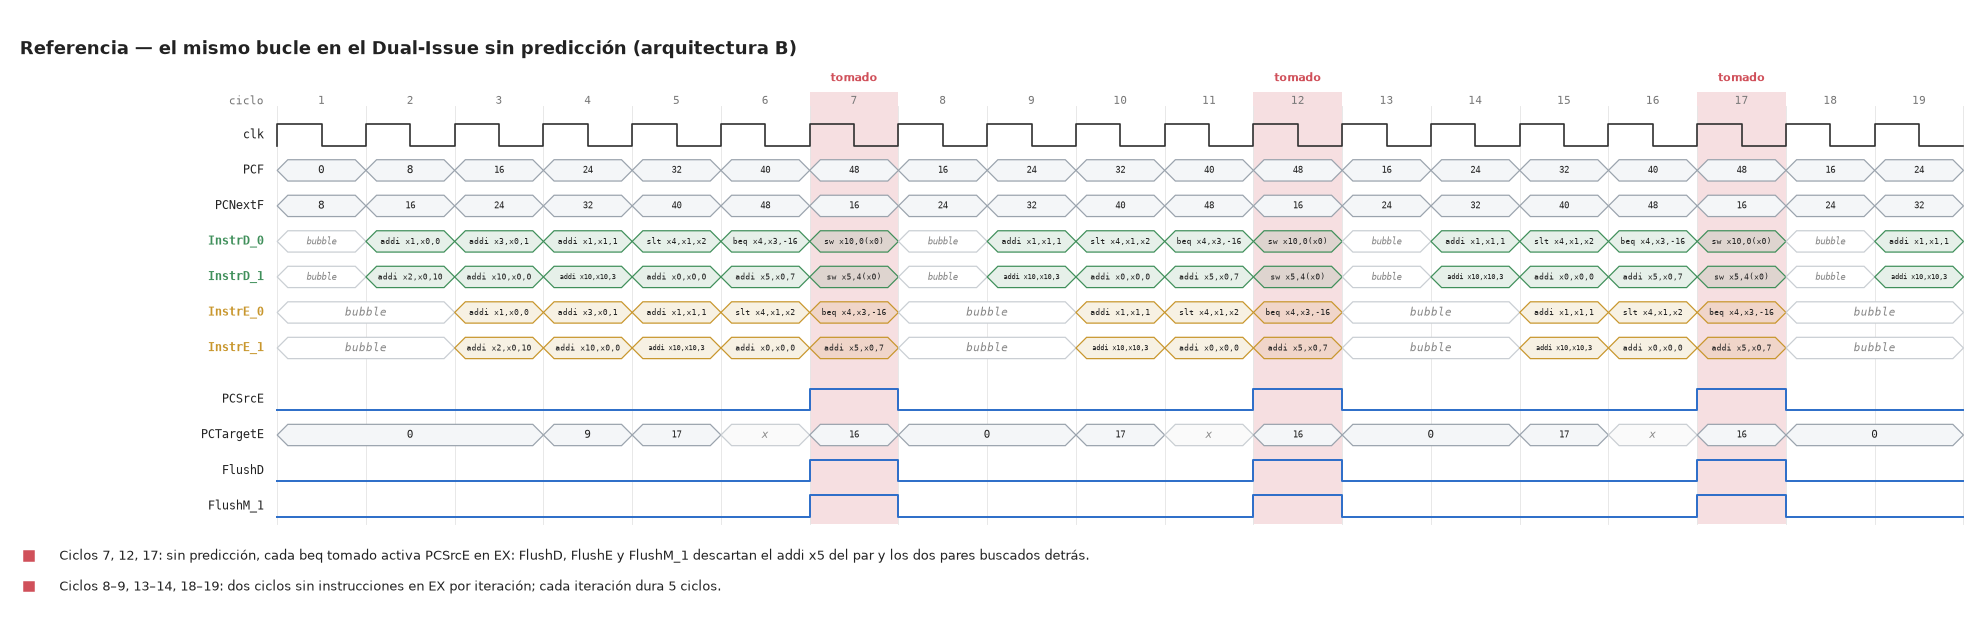
\includegraphics[width=\textwidth]{waveform-opt-slot0-B}
  \caption{Prueba 1 en B (referencia): un flush por iteración.}
  \label{fig:w-slot0-B}
\end{figure}

\begin{sidewaysfigure}
  \centering
  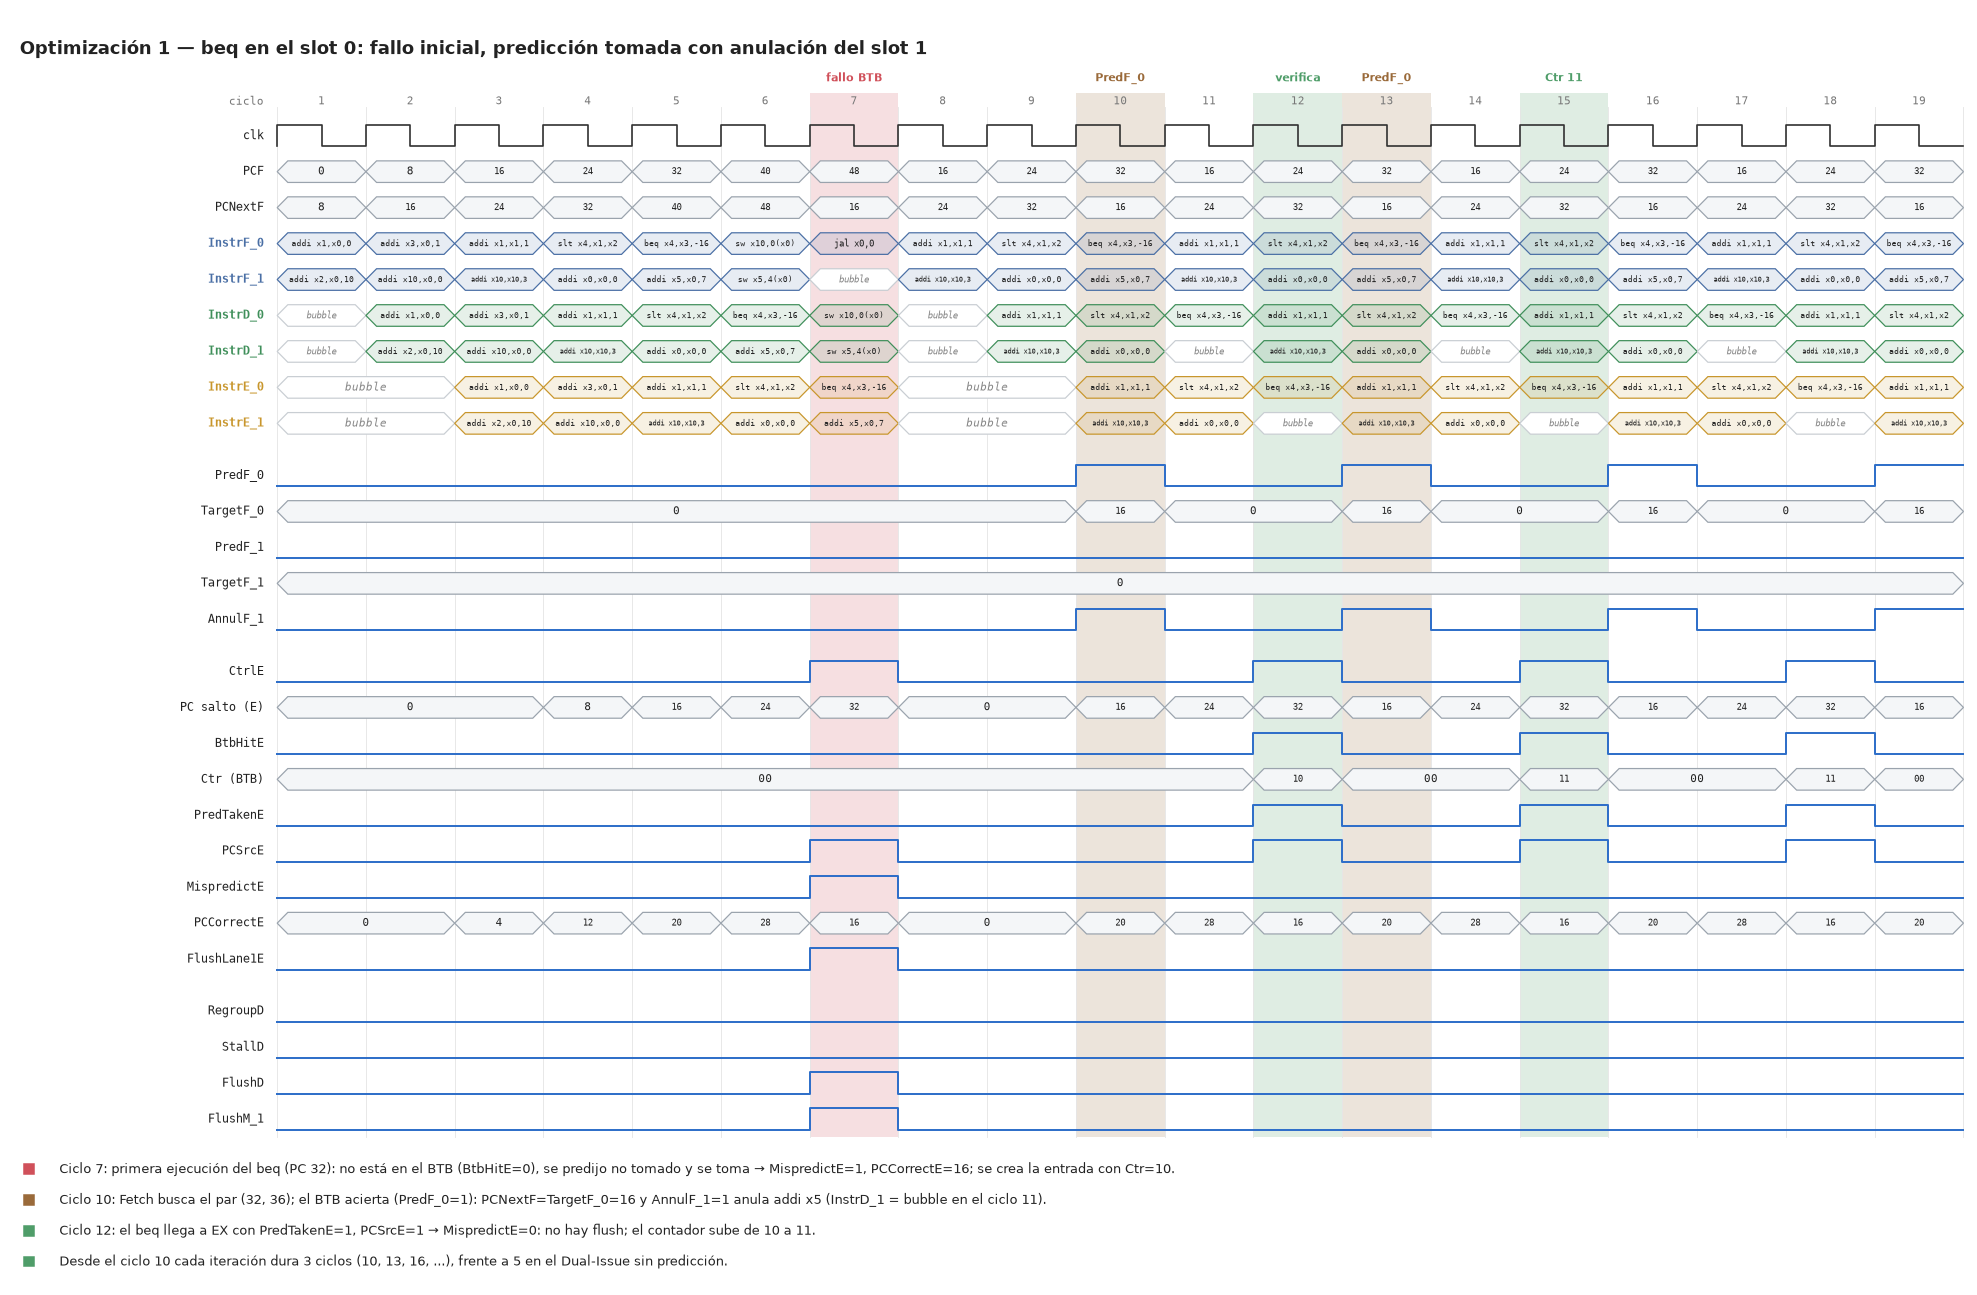
\includegraphics[width=\linewidth,height=13.5cm,keepaspectratio]{waveform-opt-slot0}
  \caption{Prueba 1 en C: primera ejecución sin entrada, predicción tomada en el slot~0 y anulación del slot~1.}
  \label{fig:w-slot0}
\end{sidewaysfigure}

\textbf{Análisis.} En el ciclo 7 el \texttt{beq} (PC 32) llega a EX por primera vez: no tiene entrada en el BTB (\sig{BtbHitE}$=0$), se había predicho no tomado y se toma, así que \sig{MispredictE}$=1$, \sig{PCCorrectE}$=16$ y se descartan Decode, Fetch y su compañero de la vía~1 (\sig{FlushM\_1}). Es el mismo costo que en B, y en ese flanco se crea la entrada con el contador en \texttt{10}.

En el ciclo 10 Fetch vuelve a buscar el par (32, 36) y el BTB acierta en el puerto 0: \sig{PredF\_0}$=1$, \sig{PCNextF}$=$\sig{TargetF\_0}$=16$ y \sig{AnnulF\_1}$=1$, de modo que en el ciclo 11 \sig{InstrD\_1} es una burbuja en lugar de \texttt{addi x5}. En el ciclo 12 el \texttt{beq} llega a EX con \sig{PredTakenE}$=1$ y se toma: \sig{MispredictE}$=0$, no hay flush y el contador pasa a \texttt{11} (en el ciclo 15 ya se lee \texttt{11}). Desde el ciclo 10 cada iteración dura 3 ciclos: los tres pares del bucle entran a EX uno detrás de otro sin huecos. En B, en cambio, cada iteración dura 5 ciclos.


\begin{figure}[H]
  \centering
  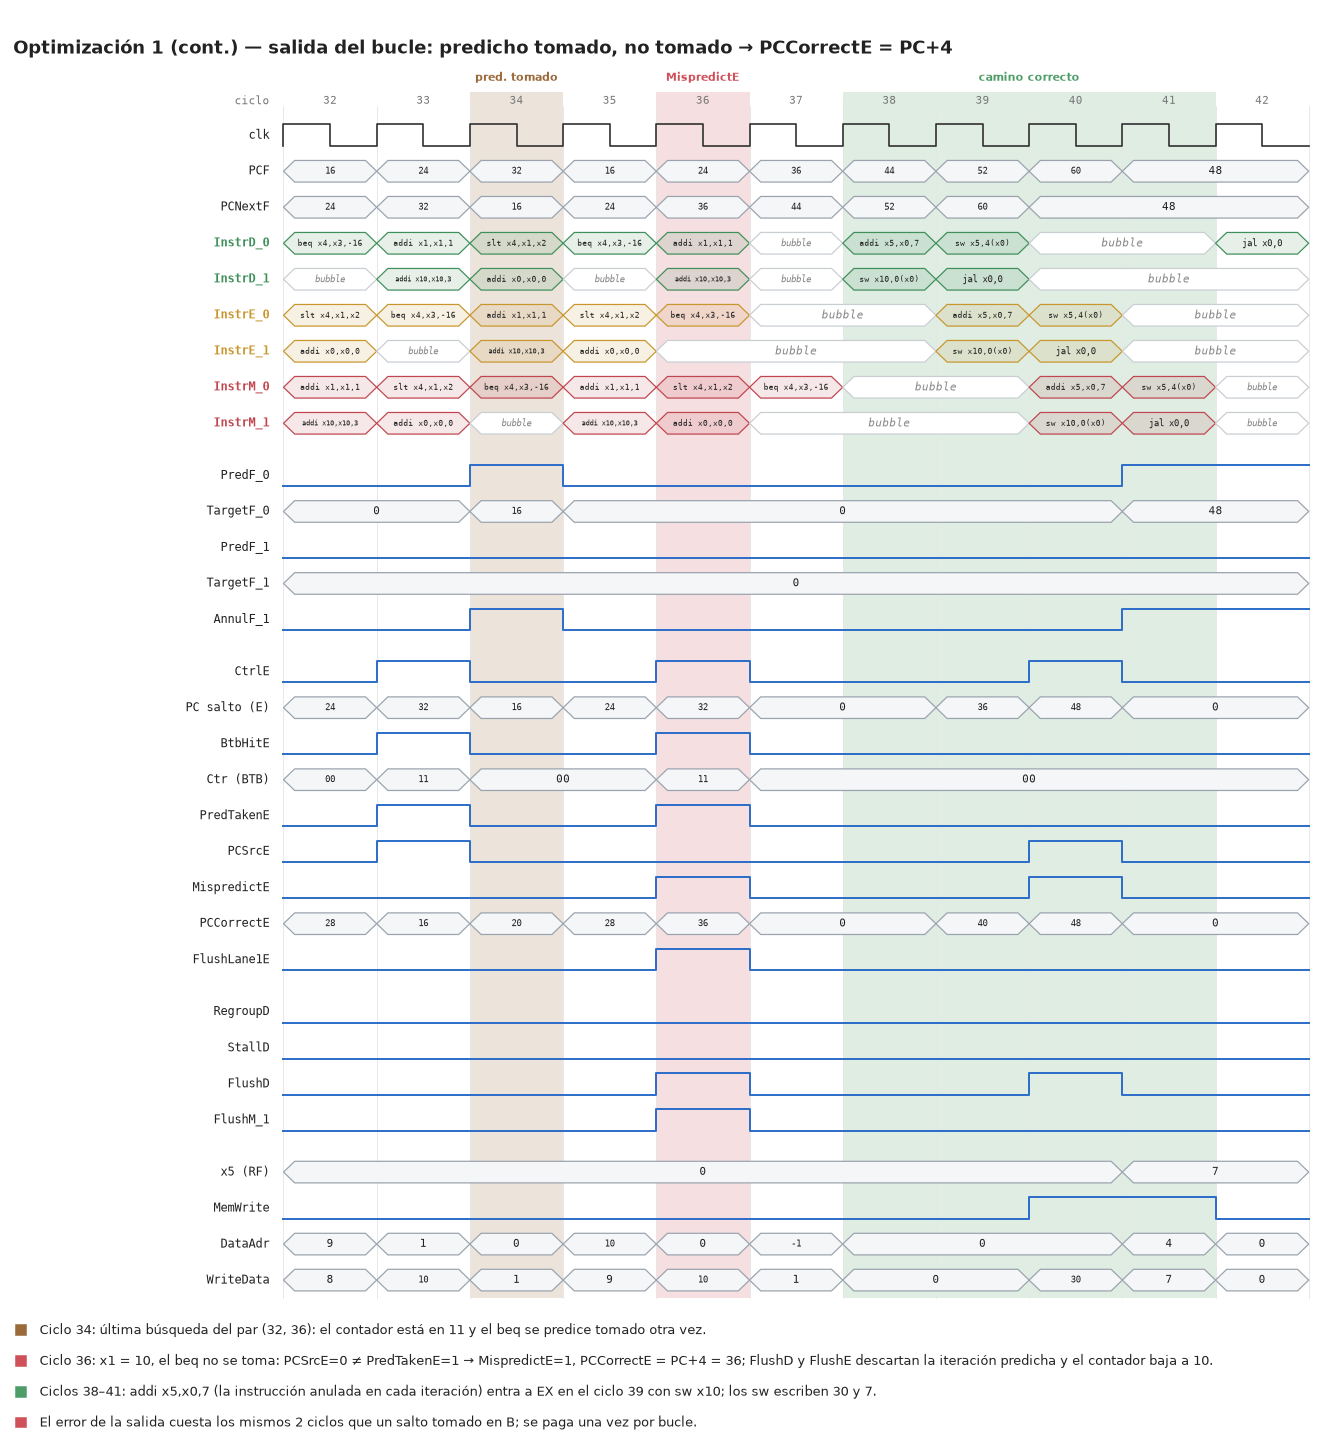
\includegraphics[width=\textwidth]{waveform-opt-slot0-exit}
  \caption{Prueba 1 en C: error de predicción a la salida del bucle.}
  \label{fig:w-slot0-exit}
\end{figure}

\textbf{Salida del bucle.} En la última iteración el contador está en \texttt{11} y el \texttt{beq} se vuelve a predecir tomado (ciclo 34), pero con x1$=10$ no se toma. En el ciclo 36 \sig{PCSrcE}$=0 \neq$ \sig{PredTakenE}$=1$: \sig{MispredictE}$=1$ y Fetch retoma en $\sig{PCCorrectE} = \sig{PCPlus4E} = 36$, la dirección del \texttt{addi x5} que se había anulado en cada iteración. El contador baja a \texttt{10}, que sigue prediciendo tomado si el bucle se vuelve a ejecutar. Los \texttt{sw} escriben \texttt{MEM[0]}$=30$ y \texttt{MEM[4]}$=7$, los valores esperados. En total hay 3 errores (primera iteración, salida y \textit{halt}) frente a 10 en B, y el programa pasa de 56 a 42 ciclos.

\FloatBarrier
% ---------------------------------------------------------------------
\subsection{Prueba 2: salto en el slot 1}


\begin{figure}[H]
  \centering
  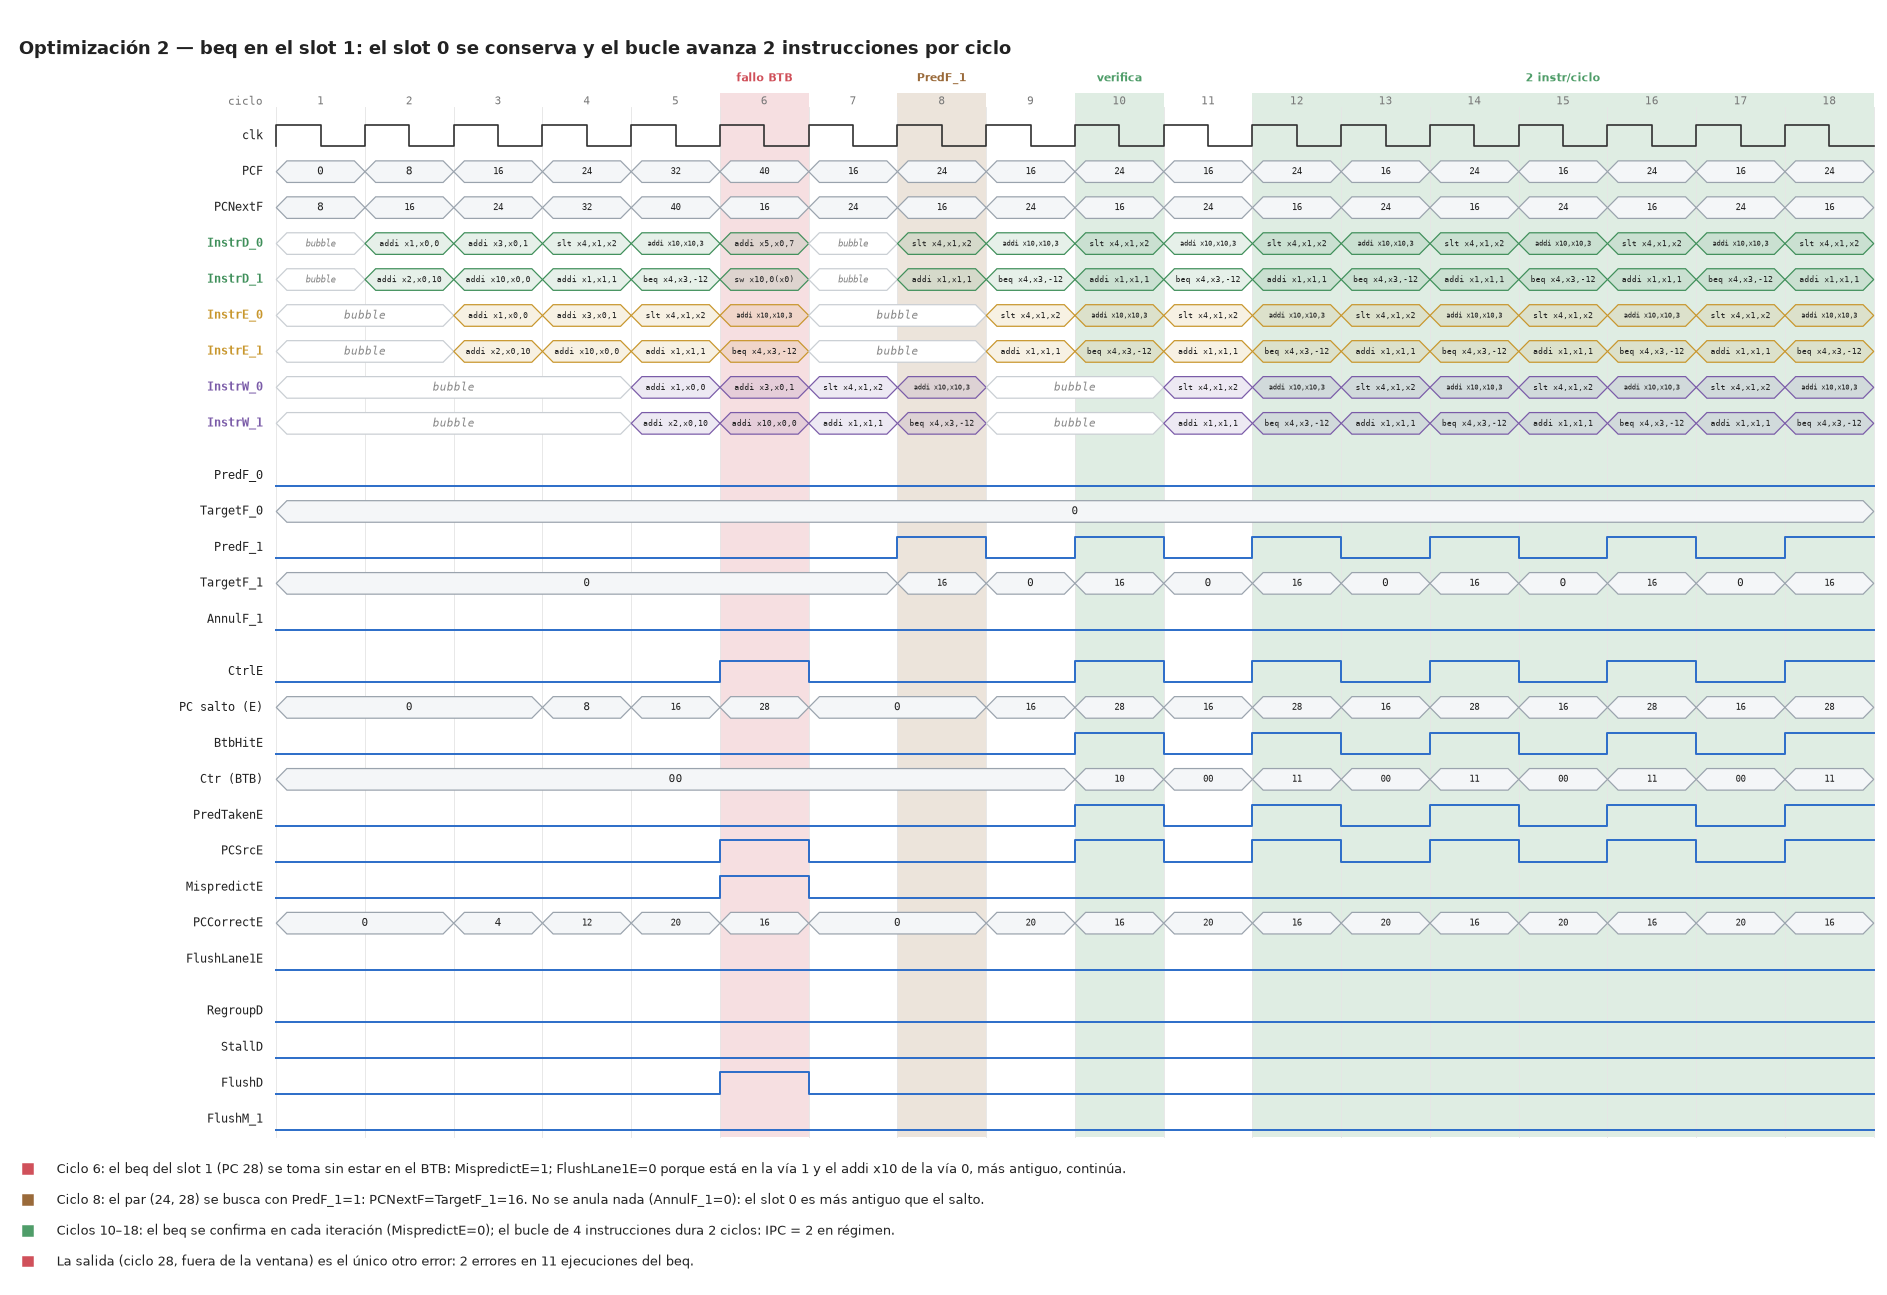
\includegraphics[width=\textwidth]{waveform-opt-slot1}
  \caption{Prueba 2 en C: salto predicho tomado en el slot~1.}
  \label{fig:w-slot1}
\end{figure}

\textbf{Análisis.} El bucle tiene cuatro instrucciones sin dependencias dentro de cada par, con el \texttt{beq} en el slot~1. En el ciclo 6 la primera ejecución falla (\sig{MispredictE}$=1$), pero \sig{FlushLane1E}$=0$ porque el salto está en la vía~1: \texttt{addi x10} (vía~0) es más antiguo y continúa. Desde el ciclo 8 el par (24, 28) se busca con \sig{PredF\_1}$=1$ y \sig{PCNextF}$=$\sig{TargetF\_1}$=16$. Esta vez no se anula nada (\sig{AnnulF\_1}$=0$): el slot~0 se ejecuta siempre. A partir del ciclo 10 el bucle avanza a dos instrucciones por ciclo, el máximo del procesador: cada iteración dura 2 ciclos. El programa pasa de 50 ciclos en B a 34 en C (speedup 1.47), con IPC 1.53.

\FloatBarrier
% ---------------------------------------------------------------------
\subsection{Prueba 3: predicción y reagrupamiento}


\begin{figure}[H]
  \centering
  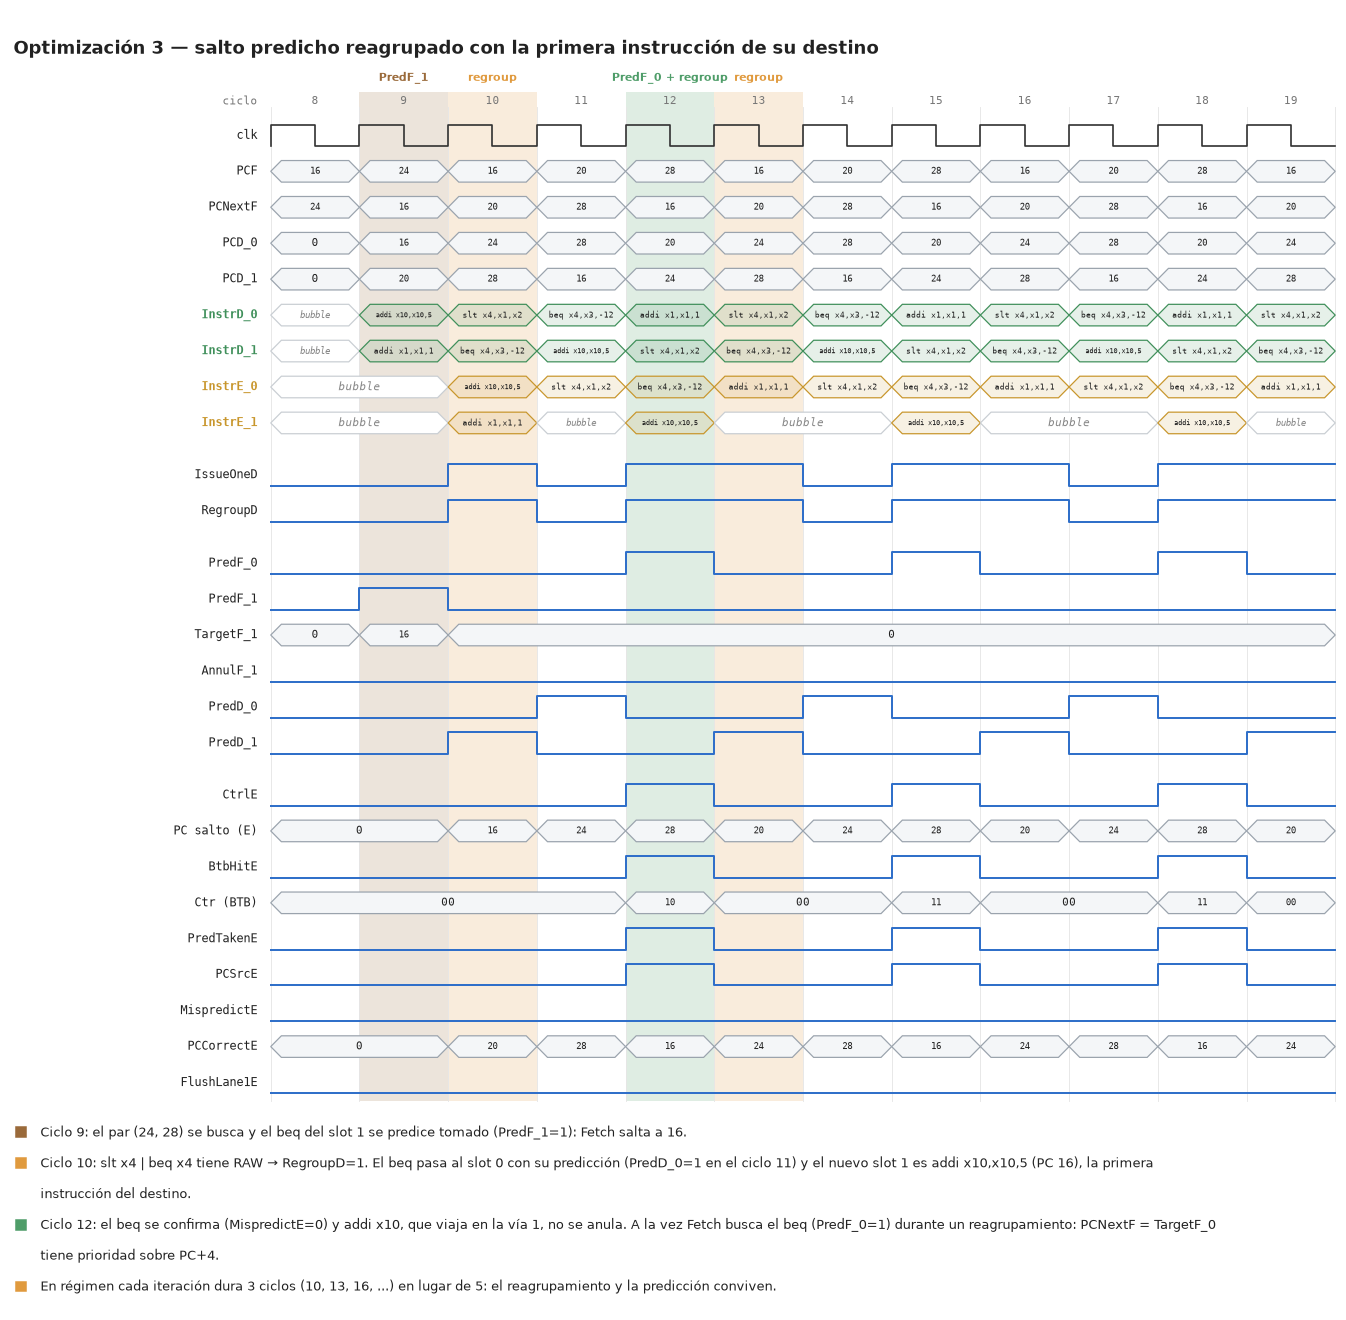
\includegraphics[width=\textwidth]{waveform-opt-regroup}
  \caption{Prueba 3 en C: el salto predicho se reagrupa con la primera instrucción de su destino.}
  \label{fig:w-regroup}
\end{figure}

\textbf{Análisis.} \texttt{slt x4} y \texttt{beq x4} están en el mismo par y tienen RAW, así que la Issue Unit solo emite el \texttt{slt}. En el ciclo 9 el par (24, 28) se busca con el \texttt{beq} predicho tomado en el slot~1 y Fetch salta a 16. En el ciclo 10 \sig{RegroupD}$=1$: el \texttt{beq} pasa al slot~0 llevando su predicción (\sig{PredD\_0}$=1$ en el ciclo 11) y el nuevo slot~1 es \texttt{addi x10,x10,5} (PC 16), la primera instrucción del destino, que es justamente la que lo sigue en el camino predicho. En el ciclo 12 el salto se confirma y ese \texttt{addi} no se anula. En ese mismo ciclo se da la combinación más delicada: Fetch busca el \texttt{beq} (\sig{PredF\_0}$=1$) mientras hay un reagrupamiento, y \sig{PCNextF}$=16$ porque \sig{PredF\_0} tiene prioridad sobre \sig{PCPlus4F}. Cada iteración dura 3 ciclos en C y 5 en B; x10$=30$ y x5$=9$ al final, como se esperaba.

\FloatBarrier
% ---------------------------------------------------------------------
\subsection{Prueba 4: jal en el BTB}


\begin{sidewaysfigure}
  \centering
  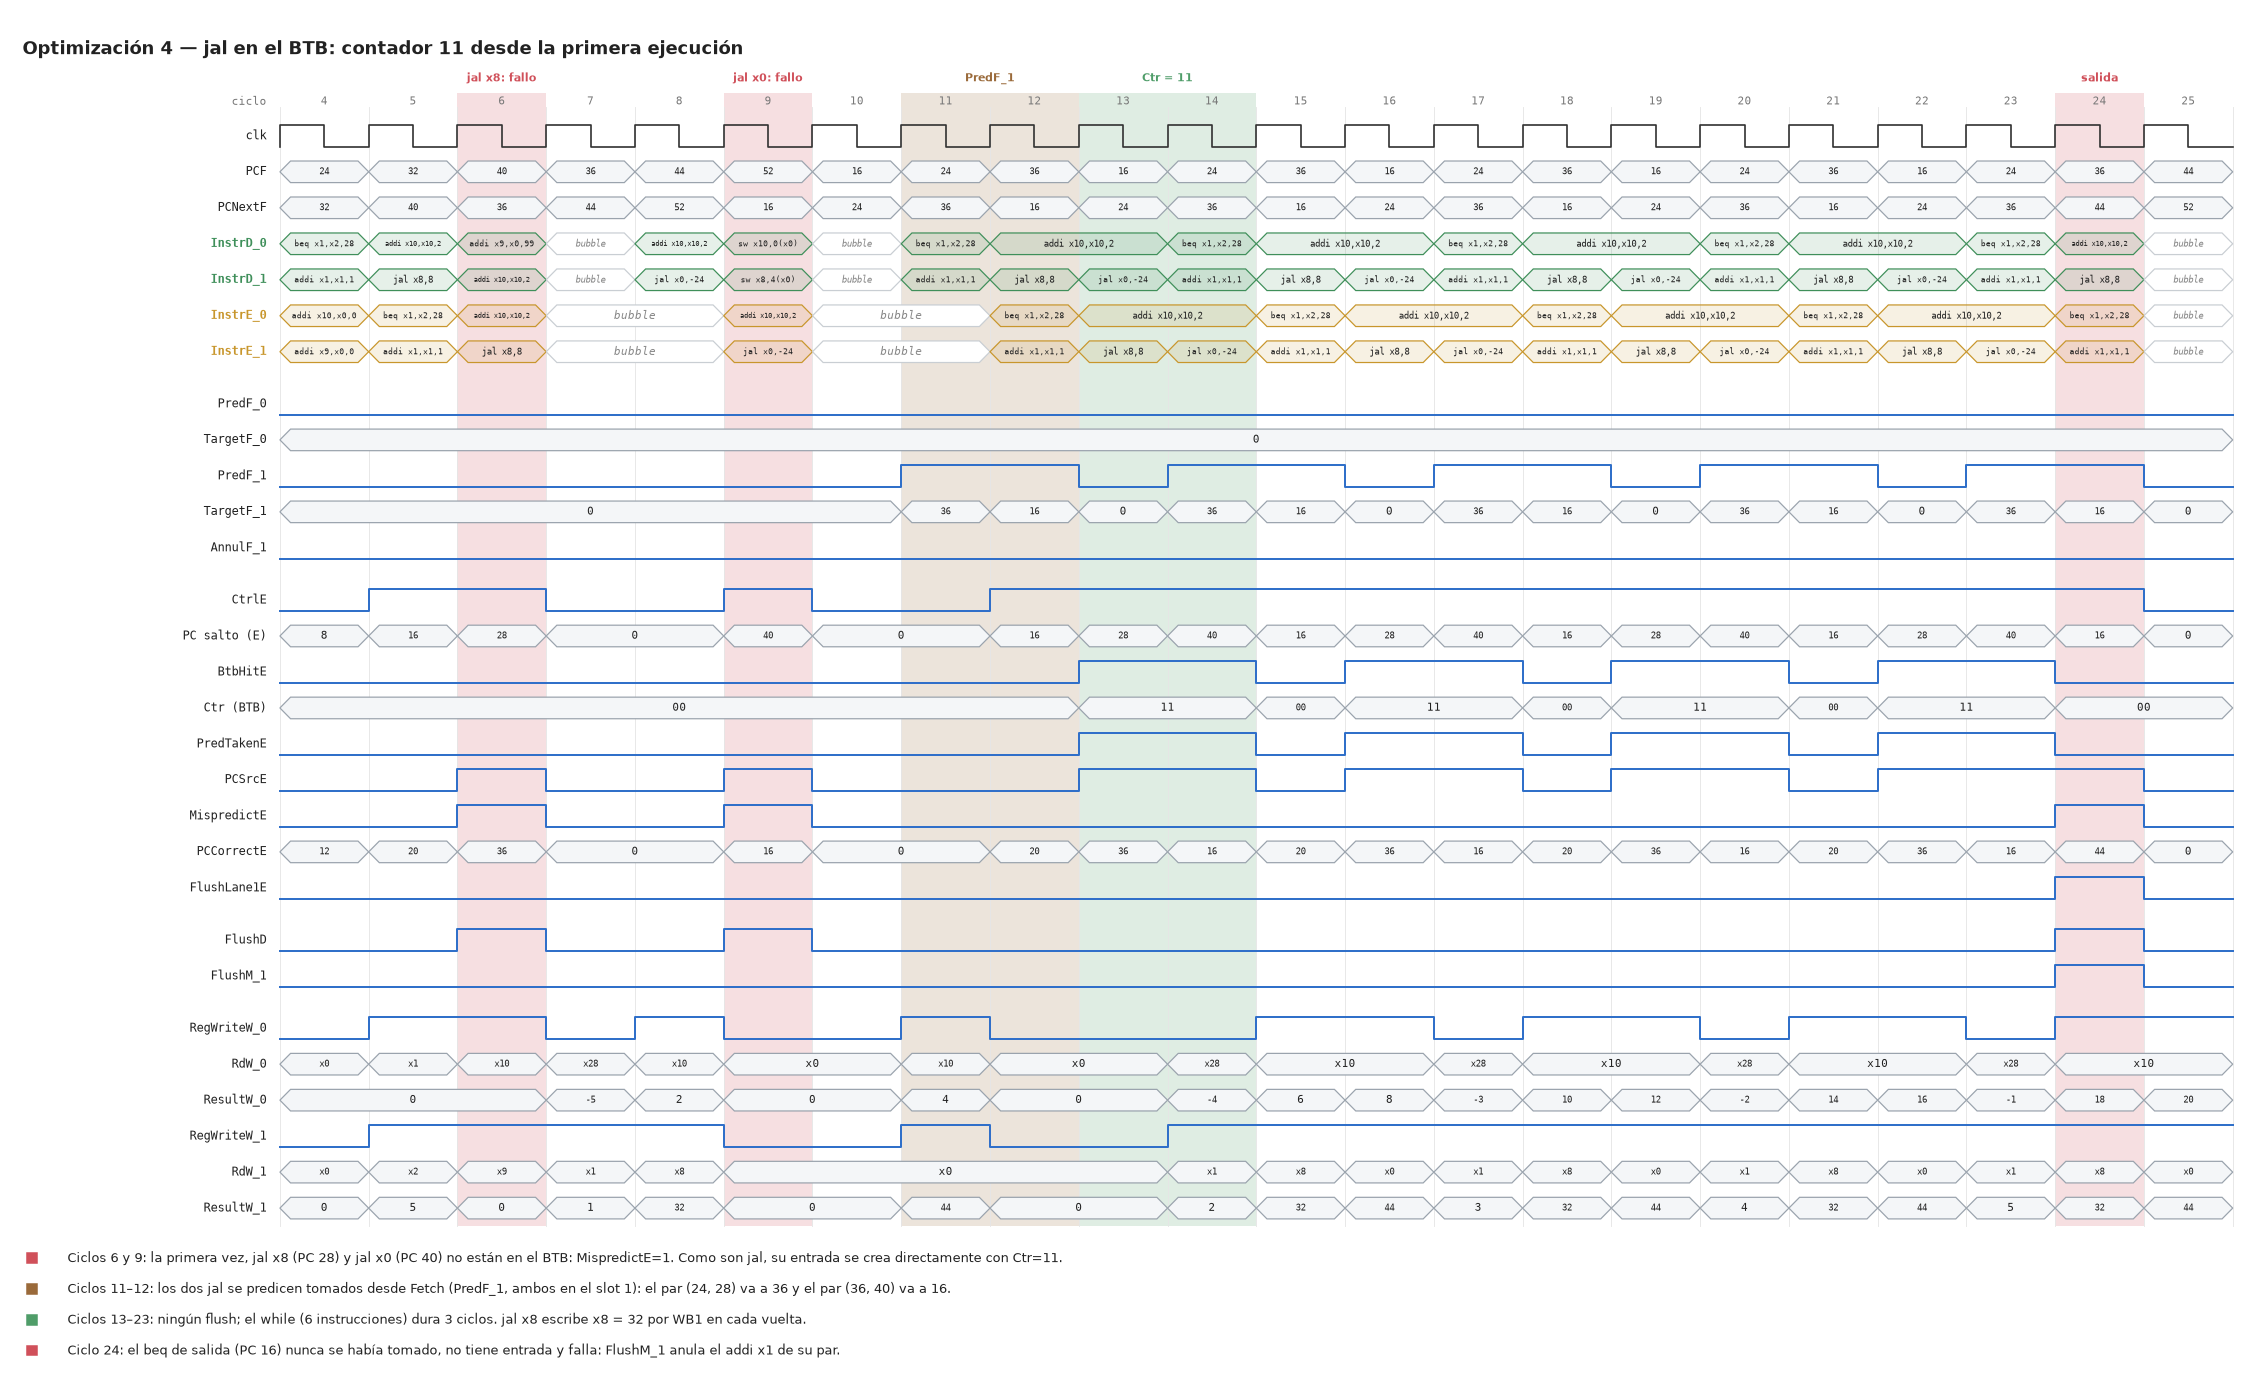
\includegraphics[width=\linewidth,height=13.5cm,keepaspectratio]{waveform-opt-jal}
  \caption{Prueba 4 en C: dos \texttt{jal} aprendidos por el BTB y un \texttt{beq} de salida que nunca se había tomado.}
  \label{fig:w-jal}
\end{sidewaysfigure}


\textbf{Análisis.} La primera vez, \texttt{jal x8} (PC 28) y \texttt{jal x0} (PC 40) fallan (ciclos 6 y 9) y sus entradas se crean con el contador en \texttt{11}. Desde los ciclos 11--12 ambos se predicen tomados en Fetch, los dos en el slot~1: el par (24, 28) va a 36 y el par (36, 40) va a 16. El \textit{while} de seis instrucciones dura 3 ciclos por vuelta, sin ningún flush entre los ciclos 13 y 23, y \texttt{jal x8} escribe su dirección de retorno x8$=32$ por la vía~1 (\sig{RdW\_1}, \sig{ResultW\_1}) en cada vuelta. El \texttt{beq} de salida (PC 16) no se tomó nunca antes, no tiene entrada y falla en el ciclo 24; como está en la vía~0, \sig{FlushM\_1} anula el \texttt{addi x1} de su par. El \texttt{addi x9,x0,99} saltado nunca se ejecuta: x9$=0$.

\FloatBarrier
% ---------------------------------------------------------------------
\subsection{Prueba 5: load-use detrás de un salto bien predicho}


\begin{figure}[H]
  \centering
  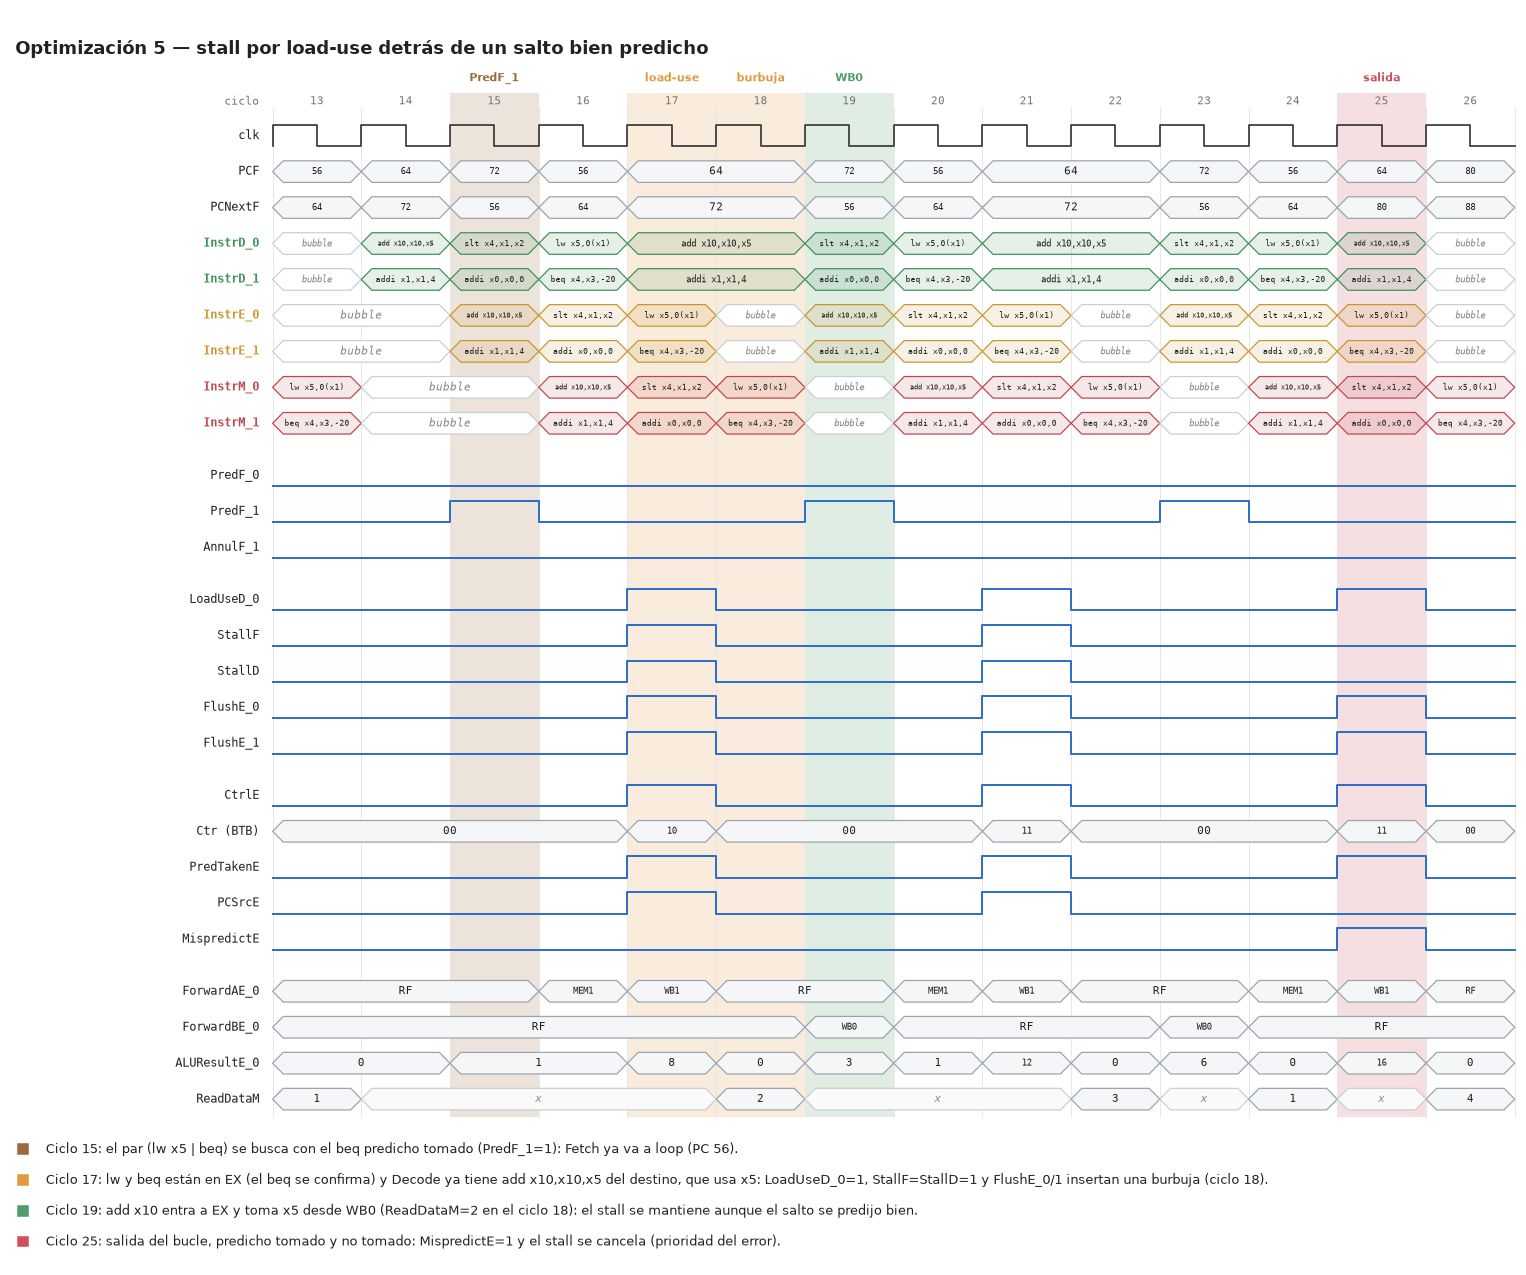
\includegraphics[width=\textwidth]{waveform-opt-loaduse}
  \caption{Prueba 5 en C: el stall por load-use se mantiene aunque el salto se haya predicho bien.}
  \label{fig:w-loaduse}
\end{figure}

\textbf{Análisis.} El par (\texttt{lw x5} | \texttt{beq}) se emite junto y el \texttt{beq} se predice tomado (ciclo 15), así que cuando ambos están en EX (ciclo 17) Decode ya contiene el par del destino, cuyo \texttt{add x10,x10,x5} usa el registro que carga el \texttt{lw}. Con predicción este caso es nuevo: en B ese par todavía no habría llegado. Como no hay error de predicción, \sig{LoadUseD\_0} detiene el par un ciclo (\sig{StallF}, \sig{StallD}, burbujas en el ciclo 18), y en el ciclo 19 \texttt{add x10} toma x5 por WB0. En el ciclo 25, a la salida, el \texttt{beq} falla y el stall se cancela, porque un error de predicción tiene prioridad: el par de Decode es del camino incorrecto. El resultado es \texttt{MEM[0]}$=10$, igual al esperado.

\FloatBarrier
% ---------------------------------------------------------------------
\subsection{Patrón y conflicto en el BTB}

\texttt{pred\_pattern} ejecuta un salto con patrón T, T, N: el contador oscila entre \texttt{11} y \texttt{10} y comete un error por periodo, 7 en total frente a 15 en B; cada no tomado mal predicho retoma en $\sig{PC}+4$ y ejecuta el camino no tomado (x11$=3$). \texttt{pred\_alias} pone dos saltos internos en los PC 36 y 100, que tienen el mismo índice ($36 = \texttt{00\,1001\,00}$, $100 = \texttt{01\,1001\,00}$): cada uno reemplaza la entrada del otro, así que ninguno llega a predecirse y C comete los mismos 15 errores que B. El resultado es correcto (x10$=$x11$=9$), lo que confirma que un conflicto en el BTB solo cuesta rendimiento, nunca corrección, gracias al Tag.

% =====================================================================
\section{Programas de comparación}
\label{sec:programas}

\subsection{Programa propio: ordenamiento burbuja}
\label{sec:propio}

El programa propio (\texttt{tb/programs/bench/bubble\_sort.s}) tiene cuatro partes:
\begin{enumerate}
    \item \textbf{Generación}: llena un arreglo de 16 palabras con la secuencia pseudoaleatoria $x \leftarrow (5x+3) \bmod 64$, $x_0 = 7$, calculando $5x$ con sumas (el procesador no tiene multiplicación).
    \item \textbf{Ordenamiento burbuja}: dos bucles anidados; el interno carga $a[j]$ y $a[j+1]$, los compara y los intercambia si están desordenados.
    \item \textbf{Suma de verificación}: suma el arreglo con dos acumuladores y un bucle desenrollado por 2, y cuenta las inversiones (que deben ser 0).
    \item \textbf{Resultados}: guarda la suma (328), las inversiones (0) y el número de intercambios (62).
\end{enumerate}

\noindent\begin{minipage}{\linewidth}
\lstinputlisting[style=programa,firstline=21,lastline=30,firstnumber=21,caption={Bucle interno del ordenamiento (\texttt{tb/programs/bench/bubble\_sort.s}, líneas 21--30).},label={lst:bubble}]{../../tb/programs/bench/bubble_sort.s}
\end{minipage}

Se eligió porque combina los factores que afectan al Dual-Issue y a la optimización, y no es una secuencia trivial de operaciones independientes:
\begin{itemize}
    \item \textbf{Paralelismo de instrucciones}: los dos \texttt{lw} del bucle interno, el incremento de \texttt{j} y las dos comparaciones son independientes entre sí; la suma de verificación usa dos acumuladores precisamente para que haya pares emitibles.
    \item \textbf{Dependencias y recursos}: cargas seguidas de comparaciones (load-use), dos \texttt{lw} y dos \texttt{sw} consecutivos que compiten por el único puerto de memoria, y \texttt{slt} seguidos de \texttt{beq} (RAW dentro del par).
    \item \textbf{Saltos de tres tipos}: los que cierran bucles (\texttt{init}, \texttt{inner}, \texttt{outer}, \texttt{check}), que el predictor aprende; y el salto del intercambio (\texttt{beq x15,x0,noswap}), que depende de los datos y no tiene un patrón regular. Esto permite ver dónde la predicción ayuda y dónde no.
\end{itemize}

\noindent Su resultado es verificable: el arreglo final \texttt{MEM[0..60]} $=$ 1, 2, 4, 5, 8, 9, 13, 14, 15, 23, 26, 28, 38, 43, 48, 51, \texttt{MEM[256]}$=328$, \texttt{MEM[260]}$=0$ y \texttt{MEM[264]}$=62$, idéntico en A, B y C.

Se usan además dos benchmarks complementarios: \texttt{sieve} (criba de Eratóstenes hasta 200, bucles con un número de vueltas distinto por primo) y \texttt{random\_branch} (32 iteraciones con un salto que depende de un bit de la secuencia pseudoaleatoria, el caso menos favorable para el predictor).

\subsection{Programa del profesor}
\label{sec:prof}

El programa del profesor (\texttt{tb/programs/final/programa.s}) se ejecuta sin modificaciones en las tres arquitecturas. Se divide en cuatro etapas: \textbf{A} (emisión y dependencias), \textbf{B} (memoria y load-use), \textbf{C} (tres bucles: C1 con un salto hacia atrás, C2 con un salto interno que alterna, C3 con un salto interno que cambia una sola vez) y \textbf{D} (bucle con cargas y un salto que depende de los datos, más saltos hacia adelante).

\paragraph{Comprobación de las etapas.} \texttt{final\_tb.v} considera que una etapa termina cuando su última instrucción, el \texttt{sw} que la cierra (\texttt{sw x10,8(x1)}, \texttt{sw x18,20(x1)}, \texttt{sw x24,32(x1)} y \texttt{sw x31,52(x1)}), llega a WB. En ese ciclo todas las instrucciones anteriores ya escribieron registros y memoria, y el testbench compara los 31 registros y las 14 palabras desde \texttt{x1}$=1536$ con el estado de referencia del enunciado (registros no indicados $= 0$, palabras aún no escritas $=$ sin valor). Si una instrucción más joven de la vía~1 escribe un registro en el mismo flanco, se compara el valor previo a esa escritura, que es el estado de la etapa en orden de programa.

\begin{table}[H]
\centering
\small
\begin{tabular}{lcccccc}
\toprule
& \multicolumn{2}{c}{\textbf{A: Pipeline}} & \multicolumn{2}{c}{\textbf{B: Dual-Issue}} & \multicolumn{2}{c}{\textbf{C: Dual + BTB}} \\
\cmidrule(lr){2-3}\cmidrule(lr){4-5}\cmidrule(lr){6-7}
\textbf{Etapa} & \textbf{Ciclo} & \textbf{Estado} & \textbf{Ciclo} & \textbf{Estado} & \textbf{Ciclo} & \textbf{Estado} \\
\midrule
A & 18  & OK & 12  & OK & 12  & OK \\
B & 32  & OK & 25  & OK & 25  & OK \\
C & 362 & OK & 312 & OK & 220 & OK \\
D & 459 & OK & 387 & OK & 292 & OK \\
\bottomrule
\end{tabular}
\caption{Ciclo de cierre de cada etapa y resultado de la comparación con el estado de referencia (\texttt{final\_tb.v}).}
\label{tab:etapas}
\end{table}

Las etapas A y B no tienen saltos, por lo que B y C las ejecutan en los mismos ciclos. La diferencia aparece en la etapa C, la de los bucles: B tarda 287 ciclos y C 195. En la etapa D la mejora es pequeña (75 frente a 72 ciclos), por razones que se explican en la Sección~\ref{sec:cuando}. Las waveforms siguientes, de C, muestran los bucles C1 y C2, donde actúa la predicción.

\subsubsection{Etapa C: bucle C1, el BTB aprende el salto}

\begin{sidewaysfigure}
  \centering
  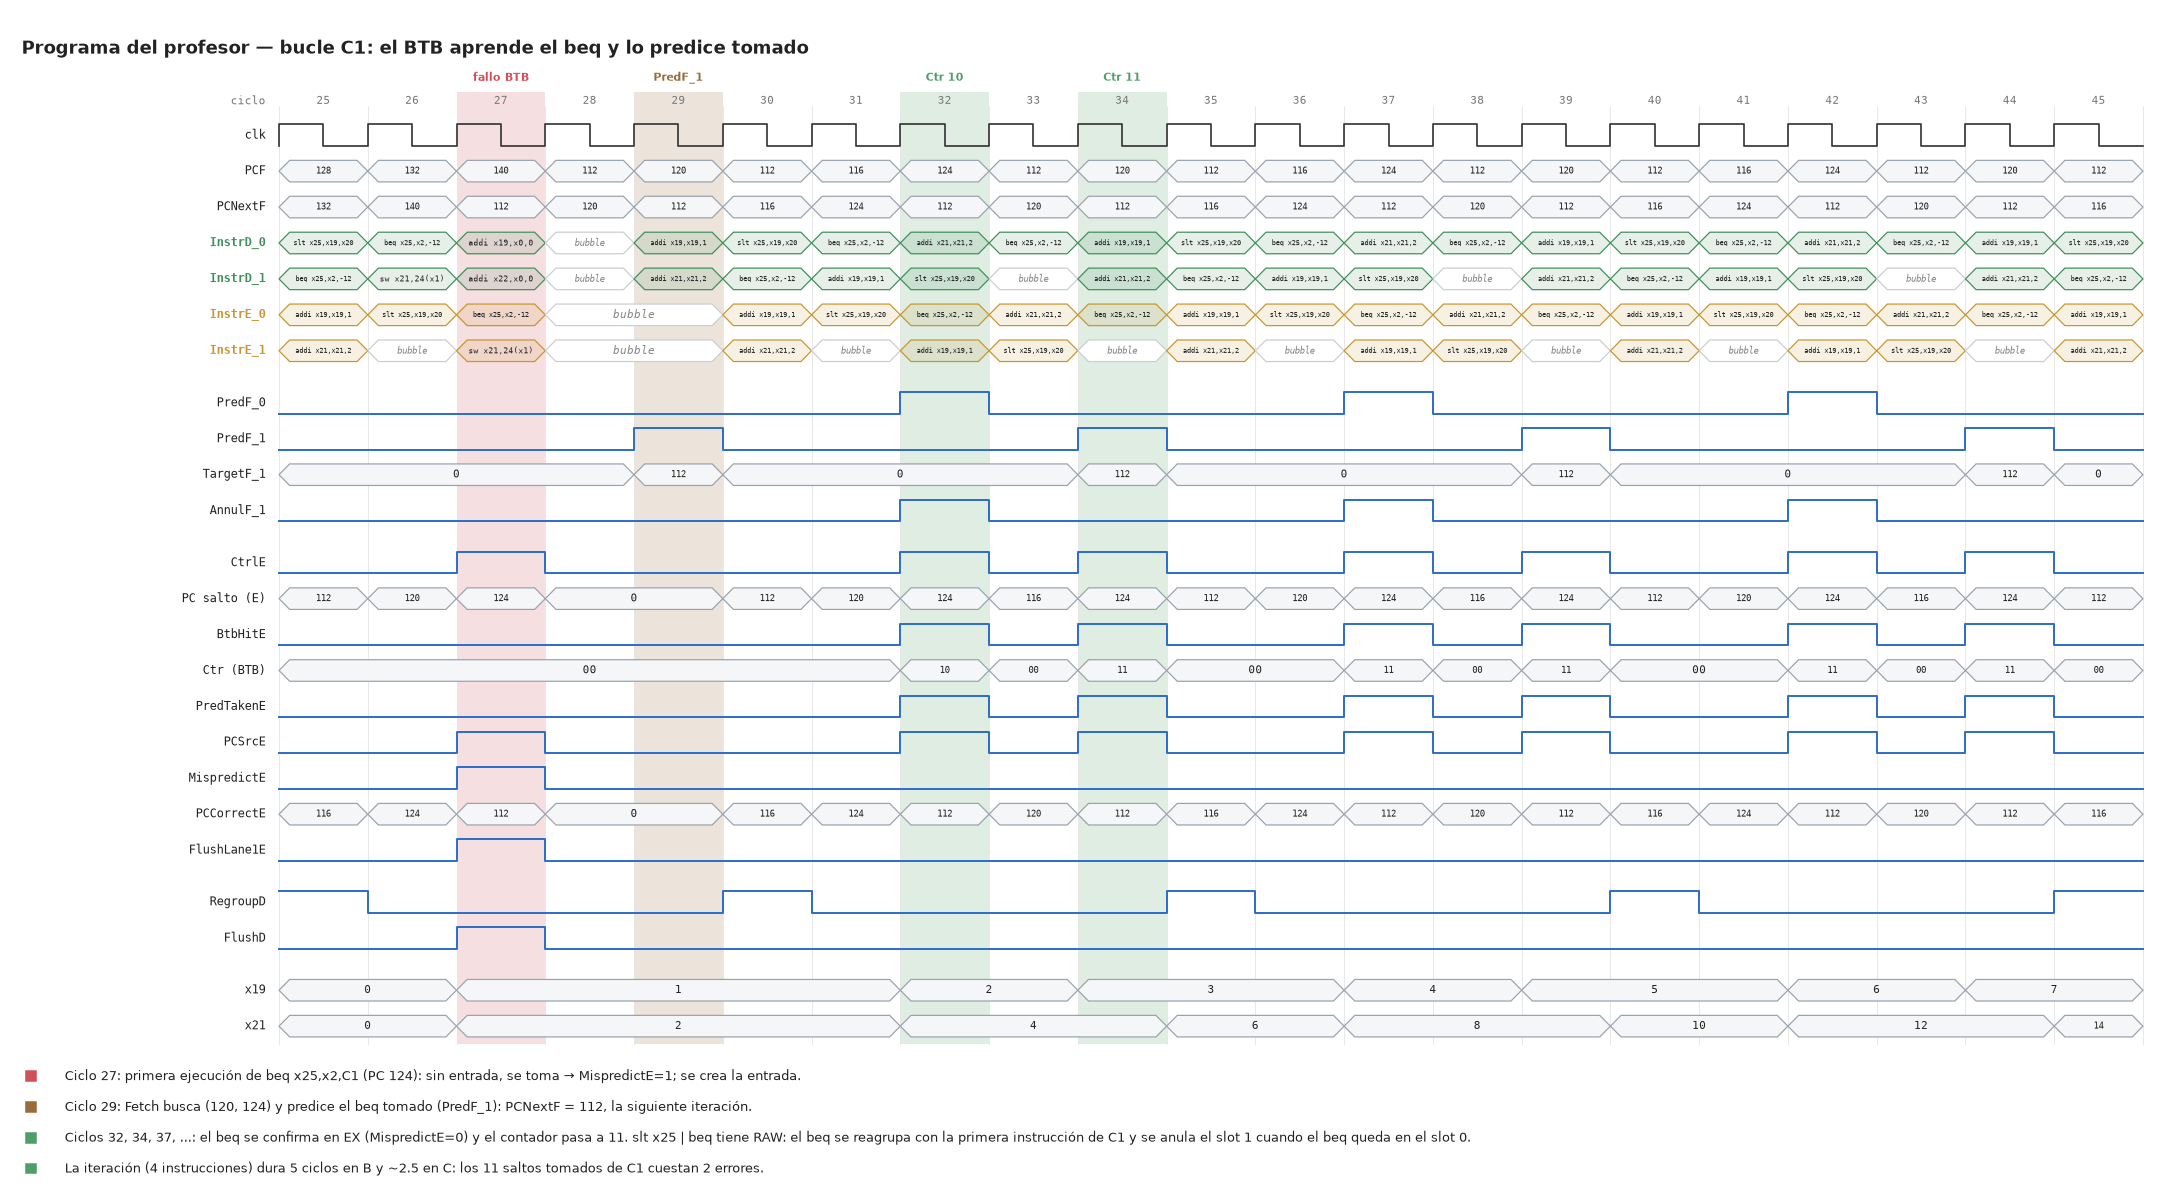
\includegraphics[width=\linewidth,height=13.5cm,keepaspectratio]{waveform-prog-C1}
  \caption{Programa del profesor en C: bucle C1.}
  \label{fig:w-C1}
\end{sidewaysfigure}

\textbf{Análisis.} El \texttt{beq x25,x2,C1} (PC 124) falla en su primera ejecución (ciclo 27) y crea su entrada. Desde el ciclo 29 Fetch lo predice tomado y \sig{PCNextF} vuelve a 112 sin esperar a EX; en los ciclos 32, 34, 37, ... la Branch Unit lo confirma (\sig{MispredictE}$=0$) y el contador sube a \texttt{11}. En C1 el \texttt{slt x25} y el \texttt{beq x25} tienen RAW, así que el \texttt{beq} se reagrupa con la primera instrucción del bucle, y cuando queda en el slot~0 de un par buscado se anula su compañero. Aun así, cada iteración de cuatro instrucciones dura 2.5 ciclos en promedio, frente a 5 en B: los 11 saltos tomados de C1 cuestan solo 2 errores (el primero y la salida).

\subsubsection{Etapa C: bucle C2, un salto que alterna}

\begin{sidewaysfigure}
  \centering
  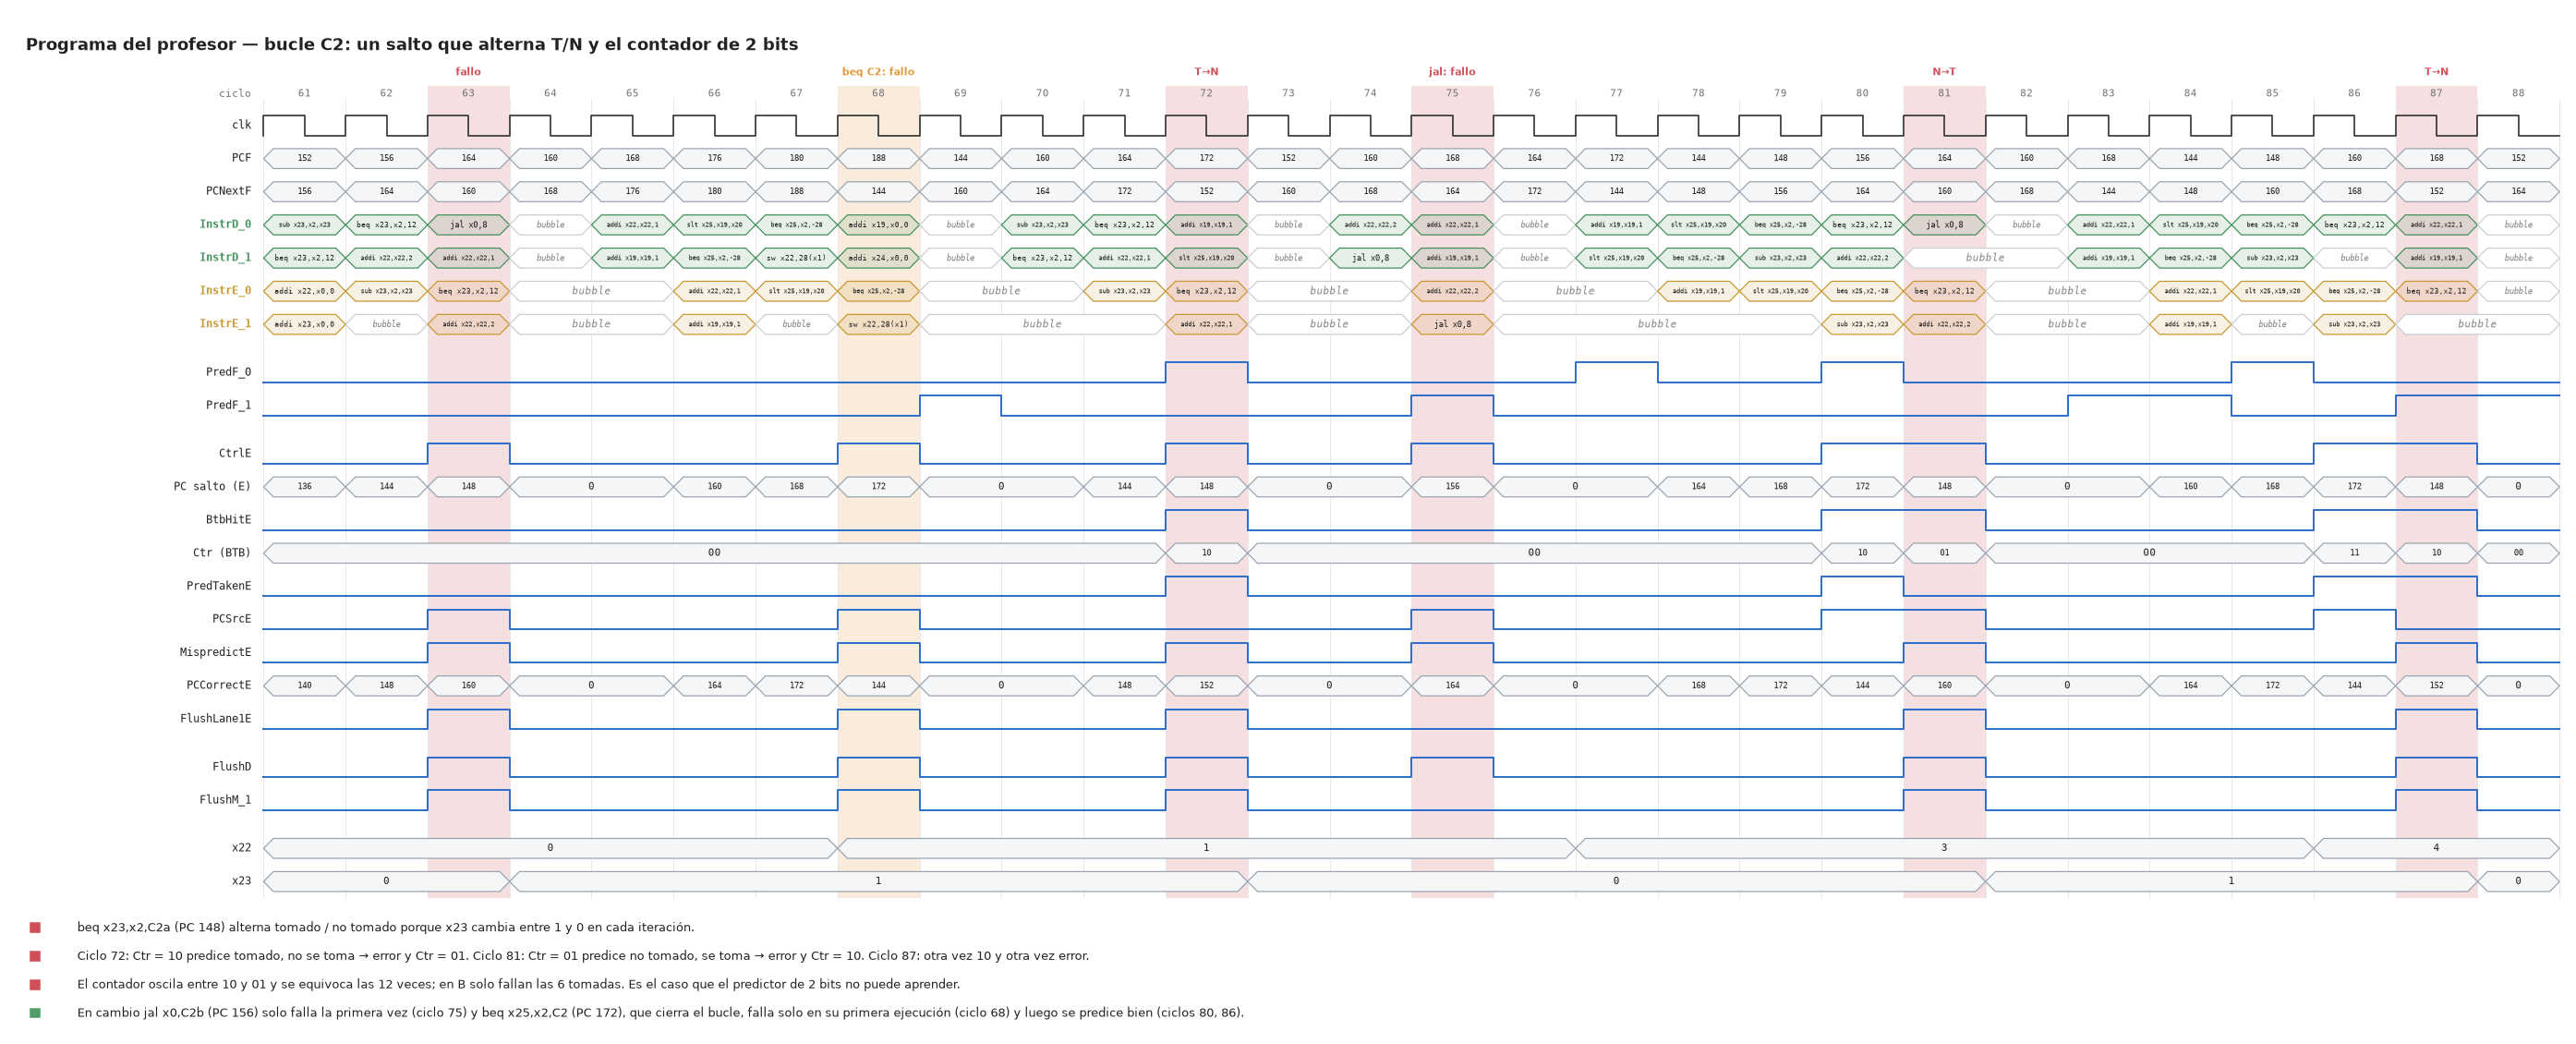
\includegraphics[width=\linewidth,height=13.5cm,keepaspectratio]{waveform-prog-C2}
  \caption{Programa del profesor en C: bucle C2, el caso desfavorable para el contador de 2 bits.}
  \label{fig:w-C2}
\end{sidewaysfigure}

\textbf{Análisis.} En C2, \texttt{sub x23,x2,x23} alterna x23 entre 1 y 0, así que \texttt{beq x23,x2,C2a} (PC 148) se toma una vez sí y otra no. En el ciclo 63 se toma sin entrada y la crea en \texttt{10}. En el ciclo 72 el contador (\texttt{10}) predice tomado y no se toma: error, y el contador baja a \texttt{01}. En el ciclo 81 el contador (\texttt{01}) predice no tomado y se toma: error, y vuelve a \texttt{10}. En el ciclo 87 se repite. El contador oscila entre los dos estados débiles y se equivoca en las 12 ejecuciones, mientras que en B solo fallan las 6 tomadas: para este salto la predicción es \emph{peor} que no predecir. En cambio, el \texttt{jal x0,C2b} (PC 156) solo falla la primera vez (ciclo 75), y el \texttt{beq} que cierra el bucle (PC 172) falla en su primera ejecución (ciclo 68) y después se predice bien (ciclos 80, 86). En el bucle C3, el salto interno se toma en las 6 primeras iteraciones y no en las 6 siguientes: el contador solo se equivoca al cambiar (3 errores frente a 6 en B).

\FloatBarrier
% =====================================================================
\section{Comparación cuantitativa}
\label{sec:comp}

\subsection{Metodología}

Las tres arquitecturas se simulan con Icarus Verilog con el mismo testbench, los mismos archivos \texttt{.mem} y los mismos datos. El ciclo 1 es el primero después del reset. Para el programa del profesor, como pide el enunciado, se excluye el bucle final \texttt{fin}: la medición termina cuando la última instrucción de la etapa D (\texttt{sw x31,52(x1)}) llega a WB, y el \texttt{jal x0,fin} no se cuenta como instrucción retirada. Para los demás programas la medición termina cuando el \textit{halt} llega a WB y este cuenta como instrucción, el mismo criterio de E2. Se supone el mismo periodo de reloj en las tres arquitecturas:
\begin{gather*}
\text{IPC} = \frac{\text{instrucciones retiradas}}{\text{ciclos}}, \qquad
\text{CPI} = \frac{\text{ciclos}}{\text{instrucciones retiradas}}, \\
\text{Speedup}_{X\to Y} = \frac{\text{ciclos}(X)}{\text{ciclos}(Y)}
\end{gather*}
La precisión de predicción es $1 - \text{errores}/\text{saltos ejecutados}$; en A y B todo salto tomado es un error, porque ambos predicen siempre ``no tomado''.

\subsection{Equivalencia funcional}

\texttt{run\_all.sh} ejecuta los 23 programas del repositorio (los 4 de E1, los 7 de E2, los 7 de la optimización, \texttt{loop}, los 3 benchmarks y el programa del profesor) en A, B y C y compara los 31 registros y toda la memoria de datos al final. Los 23 terminan con \textbf{OK}: las tres arquitecturas producen el mismo estado. Además, \texttt{final\_tb.v} verifica las cuatro etapas del programa del profesor contra los estados de referencia (Tabla~\ref{tab:etapas}), y los programas de la optimización y los benchmarks terminan con los valores esperados de sus encabezados.

\subsection{Resultados de los dos programas}

\begin{table}[H]
\centering
\small
\setlength{\tabcolsep}{5pt}
\begin{tabular}{@{}lcccccc@{}}
\toprule
& \multicolumn{3}{c}{\textbf{Programa del profesor}} & \multicolumn{3}{c}{\textbf{Programa propio}} \\
\cmidrule(lr){2-4}\cmidrule(lr){5-7}
\textbf{Indicador} & \textbf{A} & \textbf{B} & \textbf{C} & \textbf{A} & \textbf{B} & \textbf{C} \\
\midrule
Ciclos totales & 459 & 387 & 292 & 1735 & 1421 & 1163 \\
Instrucciones retiradas & 312 & 312 & 312 & 1335 & 1335 & 1335 \\
CPI & 1.471 & 1.240 & 0.936 & 1.300 & 1.064 & 0.871 \\
IPC & 0.680 & 0.806 & 1.068 & 0.769 & 0.939 & 1.148 \\
Speedup vs. pipeline & 1.00 & 1.186 & 1.572 & 1.00 & 1.221 & 1.492 \\
Speedup vs. Dual-Issue & --- & 1.00 & 1.325 & --- & 1.00 & 1.222 \\
\midrule
Ciclos con dos instr. en EX & --- & 140 & 119 & --- & 512 & 368 \\
Ciclos con una instr. en EX & 313 & 99 & 95 & 1335 & 509 & 640 \\
Stalls por load-use & 9 & 10 & 10 & 0 & 0 & 1 \\
Reagrupamientos & --- & 99 & 73 & --- & 509 & 552 \\
Ciclos con flush (\sig{FlushD}) & 68 & 68 & 33 & 199 & 199 & 76 \\
Saltos ejecutados & 90 & 90 & 90 & 279 & 279 & 279 \\
Saltos tomados & 68 & 68 & 68 & 199 & 199 & 199 \\
Errores de predicción & 68 & 68 & 33 & 199 & 199 & 76 \\
Precisión de predicción & 24.4\,\% & 24.4\,\% & 63.3\,\% & 28.7\,\% & 28.7\,\% & 72.8\,\% \\
Aciertos en el BTB & --- & --- & 74 & --- & --- & 271 \\
\bottomrule
\end{tabular}
\caption{Resultados de A (pipeline), B (Dual-Issue) y C (Dual-Issue + BTB) en el programa del profesor y en el propio (\textit{bubble sort}). En el programa del profesor se excluye el bucle \texttt{fin}; sus métricas adicionales (debajo de la línea) se cuentan hasta que el \textit{halt} llega a WB, que en B y C coincide con el cierre de D y en A ocurre un ciclo después, e incluyen el \textit{halt} como salto. Con el \textit{halt} incluido, los ciclos del profesor son 460, 387 y 292 y el IPC 0.680, 0.809 y 1.072.}
\label{tab:prof}
\label{tab:propio}
\end{table}

\begin{table}[H]
\centering
\small
\setlength{\tabcolsep}{4pt}
\begin{tabular}{rlcccc}
\toprule
\textbf{PC} & \textbf{Salto} & \textbf{Ejec.} & \textbf{Tomados} & \textbf{Err. B} & \textbf{Err. C} \\
\midrule
\multicolumn{6}{l}{\textit{Programa del profesor}} \\
124 & \texttt{beq x25,x2,C1} (cierra C1)       & 12 & 11 & 11 & 2 \\
148 & \texttt{beq x23,x2,C2a} (alterna)        & 12 & 6  & 6  & 12 \\
156 & \texttt{jal x0,C2b}                      & 6  & 6  & 6  & 1 \\
172 & \texttt{beq x25,x2,C2} (cierra C2)       & 12 & 11 & 11 & 2 \\
196 & \texttt{beq x25,x2,C3a} (6 T, luego 6 N) & 12 & 6  & 6  & 3 \\
204 & \texttt{jal x0,C3b}                      & 6  & 6  & 6  & 1 \\
220 & \texttt{beq x25,x2,C3} (cierra C3)       & 12 & 11 & 11 & 2 \\
264 & \texttt{beq x25,x2,D2} (según los datos) & 6  & 2  & 2  & 4 \\
284 & \texttt{beq x25,x2,D1} (cierra D1)       & 6  & 5  & 5  & 2 \\
300--356 & 5 saltos de D y el \textit{halt}, una ejecución cada uno & 6 & 4 & 4 & 4 \\
    & \textbf{Total}                           & 90 & 68 & 68 & 33 \\
\midrule
\multicolumn{6}{l}{\textit{Programa propio}} \\
48  & \texttt{beq x9,x3,init}                  & 16  & 15  & 15  & 2 \\
84  & \texttt{beq x15,x0,noswap} (según los datos) & 120 & 58 & 58 & 53 \\
100 & \texttt{beq x16,x3,inner}                & 120 & 105 & 105 & 16 \\
112 & \texttt{beq x17,x3,outer}                & 15  & 14  & 14  & 2 \\
180 & \texttt{beq x9,x3,check}                 & 7   & 6   & 6   & 2 \\
220 & \textit{halt}                             & 1   & 1   & 1   & 1 \\
    & \textbf{Total}                           & 279 & 199 & 199 & 76 \\
\bottomrule
\end{tabular}
\caption{Errores de predicción por salto en B y en C (\texttt{waves/branches.py}).}
\label{tab:saltos}
\end{table}

% =====================================================================
\section{Análisis}
\label{sec:analisis}

\subsection{Dual-Issue frente al pipeline}

B es entre 1.16 y 1.39 veces más rápido que A en los programas con bucles (1.19 en el del profesor y 1.22 en el propio), y hasta 1.67 en los programas cortos de E2 con instrucciones independientes. La mejora viene de los ciclos en que entran dos instrucciones a EX: 140 de 387 en el programa del profesor y 512 de 1421 en el propio. En las etapas A y B del programa del profesor, B termina en 25 ciclos frente a 32 de A, a pesar de que la etapa B es casi secuencial.

\subsection{Por qué el IPC no llega a 2}

En C, el programa del profesor alcanza IPC 1.07 y el propio 1.15. Las causas, medidas, son:
\begin{itemize}
    \item \textbf{Dependencias RAW dentro del par.} El patrón \texttt{slt x25} $\to$ \texttt{beq x25}, presente en todos los bucles del programa del profesor, obliga a emitir solo el slot~0. Hay 73 reagrupamientos en el programa del profesor y 552 en el propio: en cada uno entra una sola instrucción a EX.
    \item \textbf{Load-use y un solo puerto de memoria.} La etapa B del profesor (11 instrucciones) tarda 13 ciclos con 3 stalls y 3 pares separados por el puerto. En el programa propio, los dos \texttt{lw} consecutivos del bucle interno nunca pueden emitirse juntos.
    \item \textbf{Saltos mal predichos.} Los 33 errores del programa del profesor cuestan 66 ciclos (23\,\% de los 292) y los 76 del propio, 152 ciclos (13\,\%).
    \item \textbf{Anulación del slot~1.} Cuando un salto predicho tomado ocupa el slot~0 del par buscado, el par sale de Fetch con una sola instrucción útil. Por eso C tiene menos ciclos con doble emisión que B (119 frente a 140 y 368 frente a 512) aunque es más rápido: en B esos ciclos ``dobles'' incluían instrucciones del camino incorrecto.
    \item \textbf{Llenado del pipeline}: 4 ciclos al inicio, poco relevantes en estos programas.
\end{itemize}

\subsection{Impacto de la optimización}

En el programa del profesor C ahorra 95 ciclos respecto a B (speedup 1.325). El desglose se obtiene de los contadores de \texttt{perf\_tb}:
\begin{itemize}
    \item \textbf{70 ciclos menos sin instrucciones en EX} (148 en B, 78 en C), exactamente $2 \times (68 - 33)$: cada error de predicción evitado ahorra los dos ciclos de flush.
    \item \textbf{25 ciclos menos con instrucciones en EX} (239 en B, 214 en C). En B entran a EX $2 \cdot 140 + 99 = 379$ instrucciones, de las cuales 66 son del camino incorrecto y se anulan después del salto; en C entran 333, con solo 20 anuladas. Con predicción, el compañero de un salto tomado se anula en Fetch y no ocupa EX; a cambio, ese par entra a EX con una sola instrucción.
\end{itemize}
En el programa propio el ahorro es de 258 ciclos (speedup 1.222): 245 ciclos menos sin instrucciones en EX ($2 \times 123$ errores evitados, menos uno por el stall que aparece en C) y 13 ciclos menos con instrucciones en EX (en C entran a EX 157 instrucciones del camino incorrecto menos, pero la anulación del slot~1 convierte muchos ciclos dobles en simples). La reducción de ciclos es mayor donde los saltos son más frecuentes y regulares: en \texttt{sieve}, con 821 saltos tomados en 3261 instrucciones, C llega a un speedup de 1.62 sobre B y 1.91 sobre A, con 92\,\% de precisión.

\subsection{Cuándo resulta útil y cuándo no}
\label{sec:cuando}

La Tabla~\ref{tab:saltos} muestra que el beneficio depende del comportamiento de cada salto:
\begin{itemize}
    \item \textbf{Útil: saltos que cierran bucles y \texttt{jal}.} El \texttt{beq} que cierra un bucle de $n$ iteraciones se toma $n-1$ veces; C se equivoca en la primera (sin entrada) y en la salida. En los cierres de C1, C2 y C3 pasa de 11 a 2 errores cada uno, y en el bucle interno del propio de 105 a 16. Los \texttt{jal} solo fallan la primera vez. Es lo que explica la reducción de la etapa C del profesor de 287 a 195 ciclos.
    \item \textbf{Útil pero no ideal: patrones con pocos cambios.} El salto de C3 cambia una vez (6 T, luego 6 N): 3 errores frente a 6. \texttt{pred\_pattern} (T, T, N) baja de 15 a 7.
    \item \textbf{Perjudicial: saltos que alternan.} El salto de C2 se toma en ejecuciones alternas y el contador oscila entre \texttt{10} y \texttt{01}: 12 errores frente a 6 en B. El salto de D1 depende de los datos (N, T, N, T, N, N) y sube de 2 a 4 errores. Para esos saltos, predecir ``no tomado'' como B es mejor que el contador.
    \item \textbf{Poco útil: saltos que dependen de los datos sin patrón.} El salto del intercambio del propio (\texttt{noswap}) baja solo de 58 a 53 errores en 120 ejecuciones, cerca del azar. En \texttt{random\_branch} el speedup sobre B es 1.32, pero proviene del salto del bucle (31 a 2 errores) y del \texttt{jal} (16 a 1); el salto aleatorio solo baja de 16 a 14 errores en 32 ejecuciones.
    \item \textbf{Sin efecto: saltos que se ejecutan una vez.} Los saltos hacia adelante de la etapa D y todos los de los programas de E1 y E2 nunca están en el BTB cuando se ejecutan: pagan lo mismo que en B. Por eso la etapa D solo baja de 75 a 72 ciclos y los programas de E1/E2 no cambian.
    \item \textbf{Sin efecto: conflictos en la tabla.} Dos saltos con el mismo índice se reemplazan mutuamente (\texttt{pred\_alias}: 15 errores en B y en C). Con 16 entradas no ocurre en los programas de comparación.
\end{itemize}

\subsection{Limitaciones}
\label{sec:limit}

\begin{itemize}
    \item \textbf{Frecuencia de reloj.} La comparación supone el mismo periodo de reloj. La predicción alarga la ruta de Fetch: \sig{PCF} $\to$ lectura del BTB (multiplexor 16:1 y comparación del Tag) $\to$ cadena de cuatro multiplexores $\to$ registro del PC. Si esa ruta pasara a ser la crítica, el tiempo real de C sería mayor que lo que indican los ciclos; no se sintetizó el diseño para medirlo.
    \item \textbf{Penalización por error.} Un error sigue costando 2 ciclos porque la verificación ocurre en Execute. Los saltos que alternan o dependen de los datos pueden empeorar respecto a B.
    \item \textbf{Primera ejecución.} Un salto que no está en el BTB se predice no tomado; los saltos que se ejecutan una sola vez no se benefician.
    \item \textbf{Slot~1 anulado.} Un salto predicho en el slot~0 desperdicia la mitad del par buscado. La optimización elimina los ciclos vacíos, pero no realinea los pares.
    \item \textbf{Costo de hardware.} 976 bits de BTB, 132 bits más en registros de pipeline, dos comparadores de 26 bits y un multiplexor de lectura de 16 entradas por puerto. El tamaño es un parámetro (\texttt{-DBTB\_IDXW}): con 8 entradas se obtienen los mismos ciclos que con 16 en todos los programas medidos (con 2 o 4 aparecen conflictos), así que 16 entradas deja margen para programas con más saltos a costa de duplicar el almacenamiento.
\end{itemize}

% =====================================================================
\section{Conclusiones}

Se implementó una predicción dinámica de saltos con un BTB de 16 entradas y un contador de 2 bits sobre el procesador Dual-Issue de E2. La predicción se hace en Fetch para las dos instrucciones del par, viaja con cada instrucción a través de los stalls y reagrupamientos y se verifica en la Branch Unit, que corrige el PC solo cuando la predicción falla. La Hazard Unit no cambió de estructura: anula instrucciones por error de predicción y no por salto tomado. Las tres arquitecturas producen el mismo estado en los 23 programas, y las cuatro etapas del programa del profesor coinciden con los estados de referencia en las tres.

En el programa del profesor, el Dual-Issue con predicción alcanza un IPC de 1.07 frente a 0.81 del Dual-Issue y 0.68 del pipeline, con speedups de 1.33 y 1.57; en el programa propio, 1.15 frente a 0.94 y 0.77, con speedups de 1.22 y 1.49. La mejora se concentra en los saltos que cierran bucles y en los \texttt{jal}, y se explica casi por completo por los errores de predicción evitados (dos ciclos por cada uno). La predicción no ayuda en los saltos que se ejecutan una sola vez ni en los que dependen de los datos, y empeora los que alternan, como el de C2. Lo que sigue separando al procesador del IPC ideal de 2 son las dependencias RAW dentro del par, el único puerto de memoria, los load-use y los errores de predicción que quedan.

\end{document}
